\chapter{Results}
\label{cha:results}

This chapter is dedicated to show the analysis' results. In favor of clarity and organization, this chapter will be divided into sections, each corresponding to a different model.The plots presented in this section were made using \textit{ad-hoc} plotting functions.

Initially the regression analysis was done in the pre-processed data presented in Table~\ref{tab:prepro-sample}, i.e. each observation corresponds to a gas exposure. It is important to remind the reader that in this data, each unique gas mixture was exposed (i.e. an exposure) twelve times: four frequency cycles through three experiment repetitions, yielding 1500 observations. Subsequently, the same analysis was conducted, but this time using the only average features of the mixture averages, shown in Table~\ref{tab:prepro-sample-unique-mixtures}.

Before beginning analysis, an assessment of correlation between features is first conducted and shown in Figure~\ref{fig:cor-mat}.

\begin{figure}[h]
	\centering
	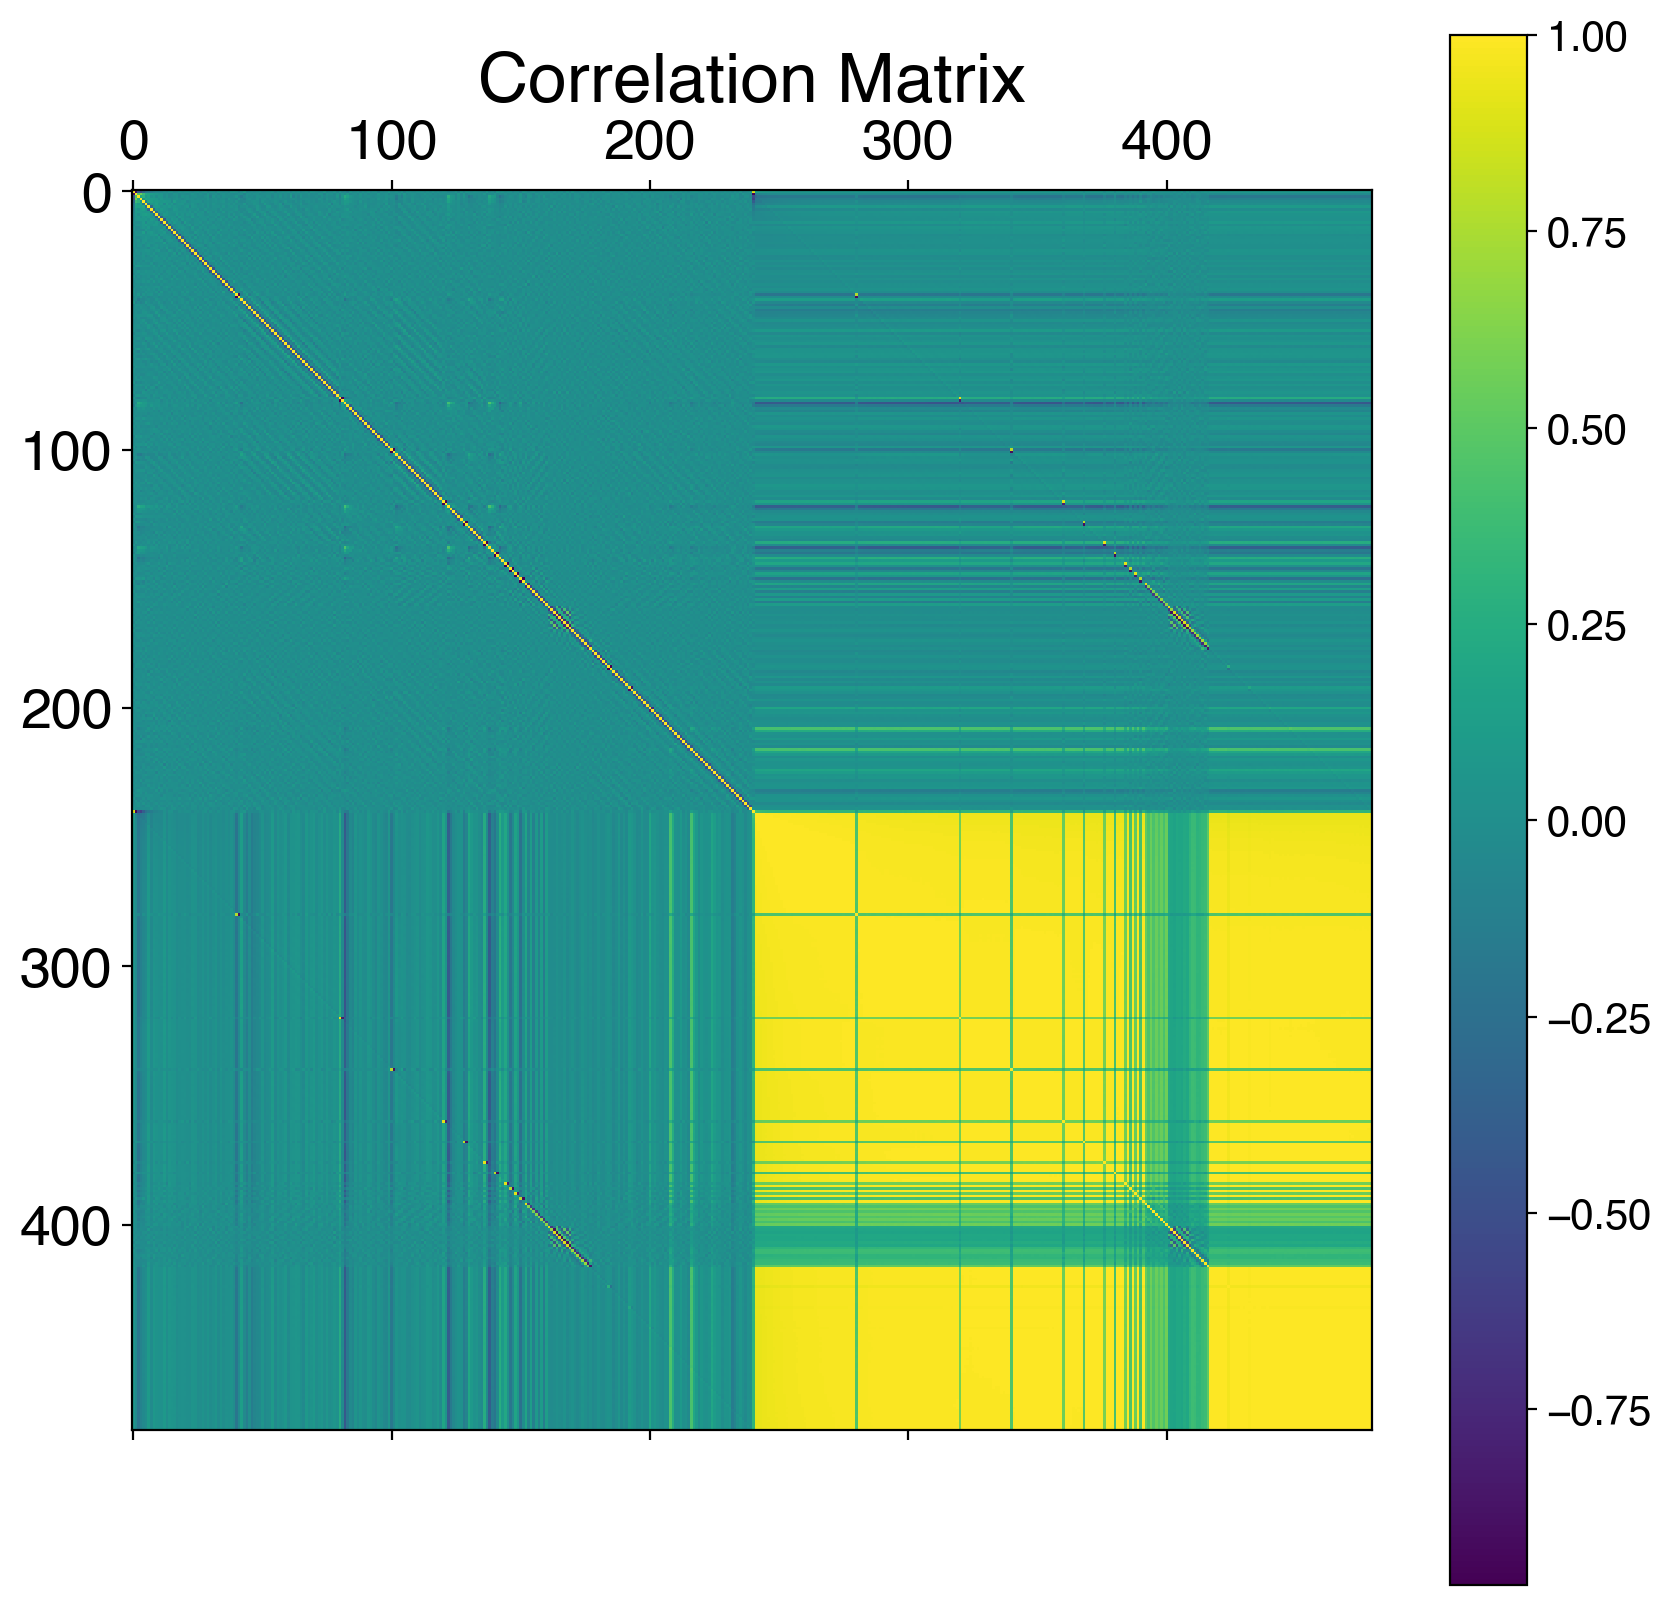
\includegraphics[width=0.35\textwidth]{../figures/correlation-matrix.png}
	\caption{Correlation matrix of features.}
	
	\label{fig:cor-mat}
\end{figure}

In Figure~\ref{fig:cor-mat}, the first, mainly green, quadrant correspond to slope features, while the fourth, mainly yellow, quadrant, averages.

\clearpage
\section{\acrlong{ols}}
\label{sec:results-ols}

As explained in Chapter~\ref{cha:methods}, \acrshort{ols} is treated here as a baseline. The actual vs. predicted plot in Figure~\ref{fig:ols-exposures} shows the predictions for both data sets.

\begin{figure}[!htb]
	\centering
	
	\begin{subfigure}[b]{1\textwidth}
		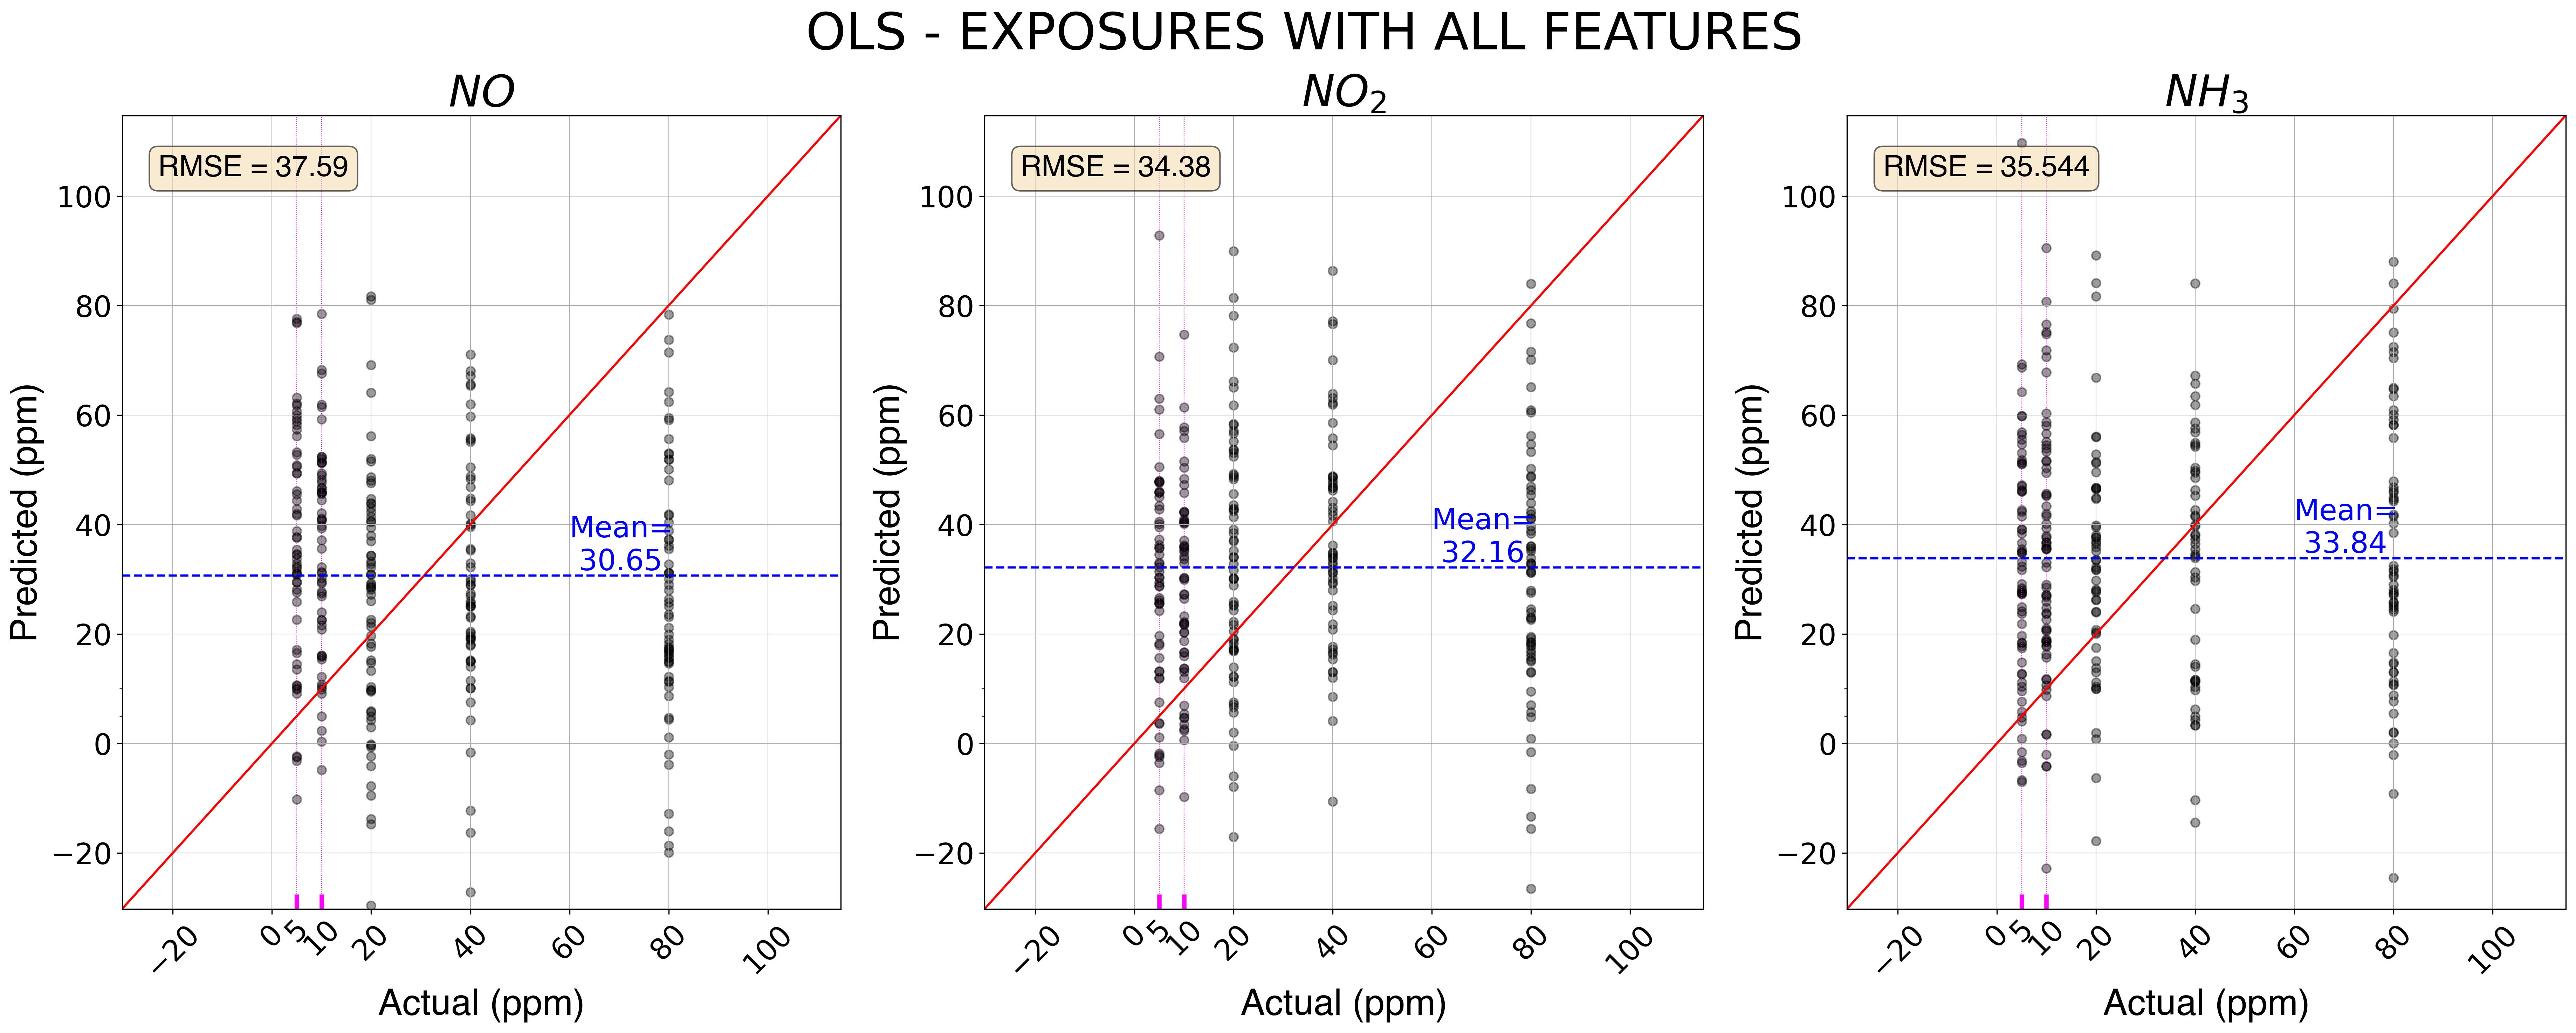
\includegraphics[width=1\linewidth]{../figures/ols-act-vs-pred.png}
		\caption{}
		\label{fig:ols-exposures} 
	\end{subfigure}
	
	\begin{subfigure}[b]{1\textwidth}
		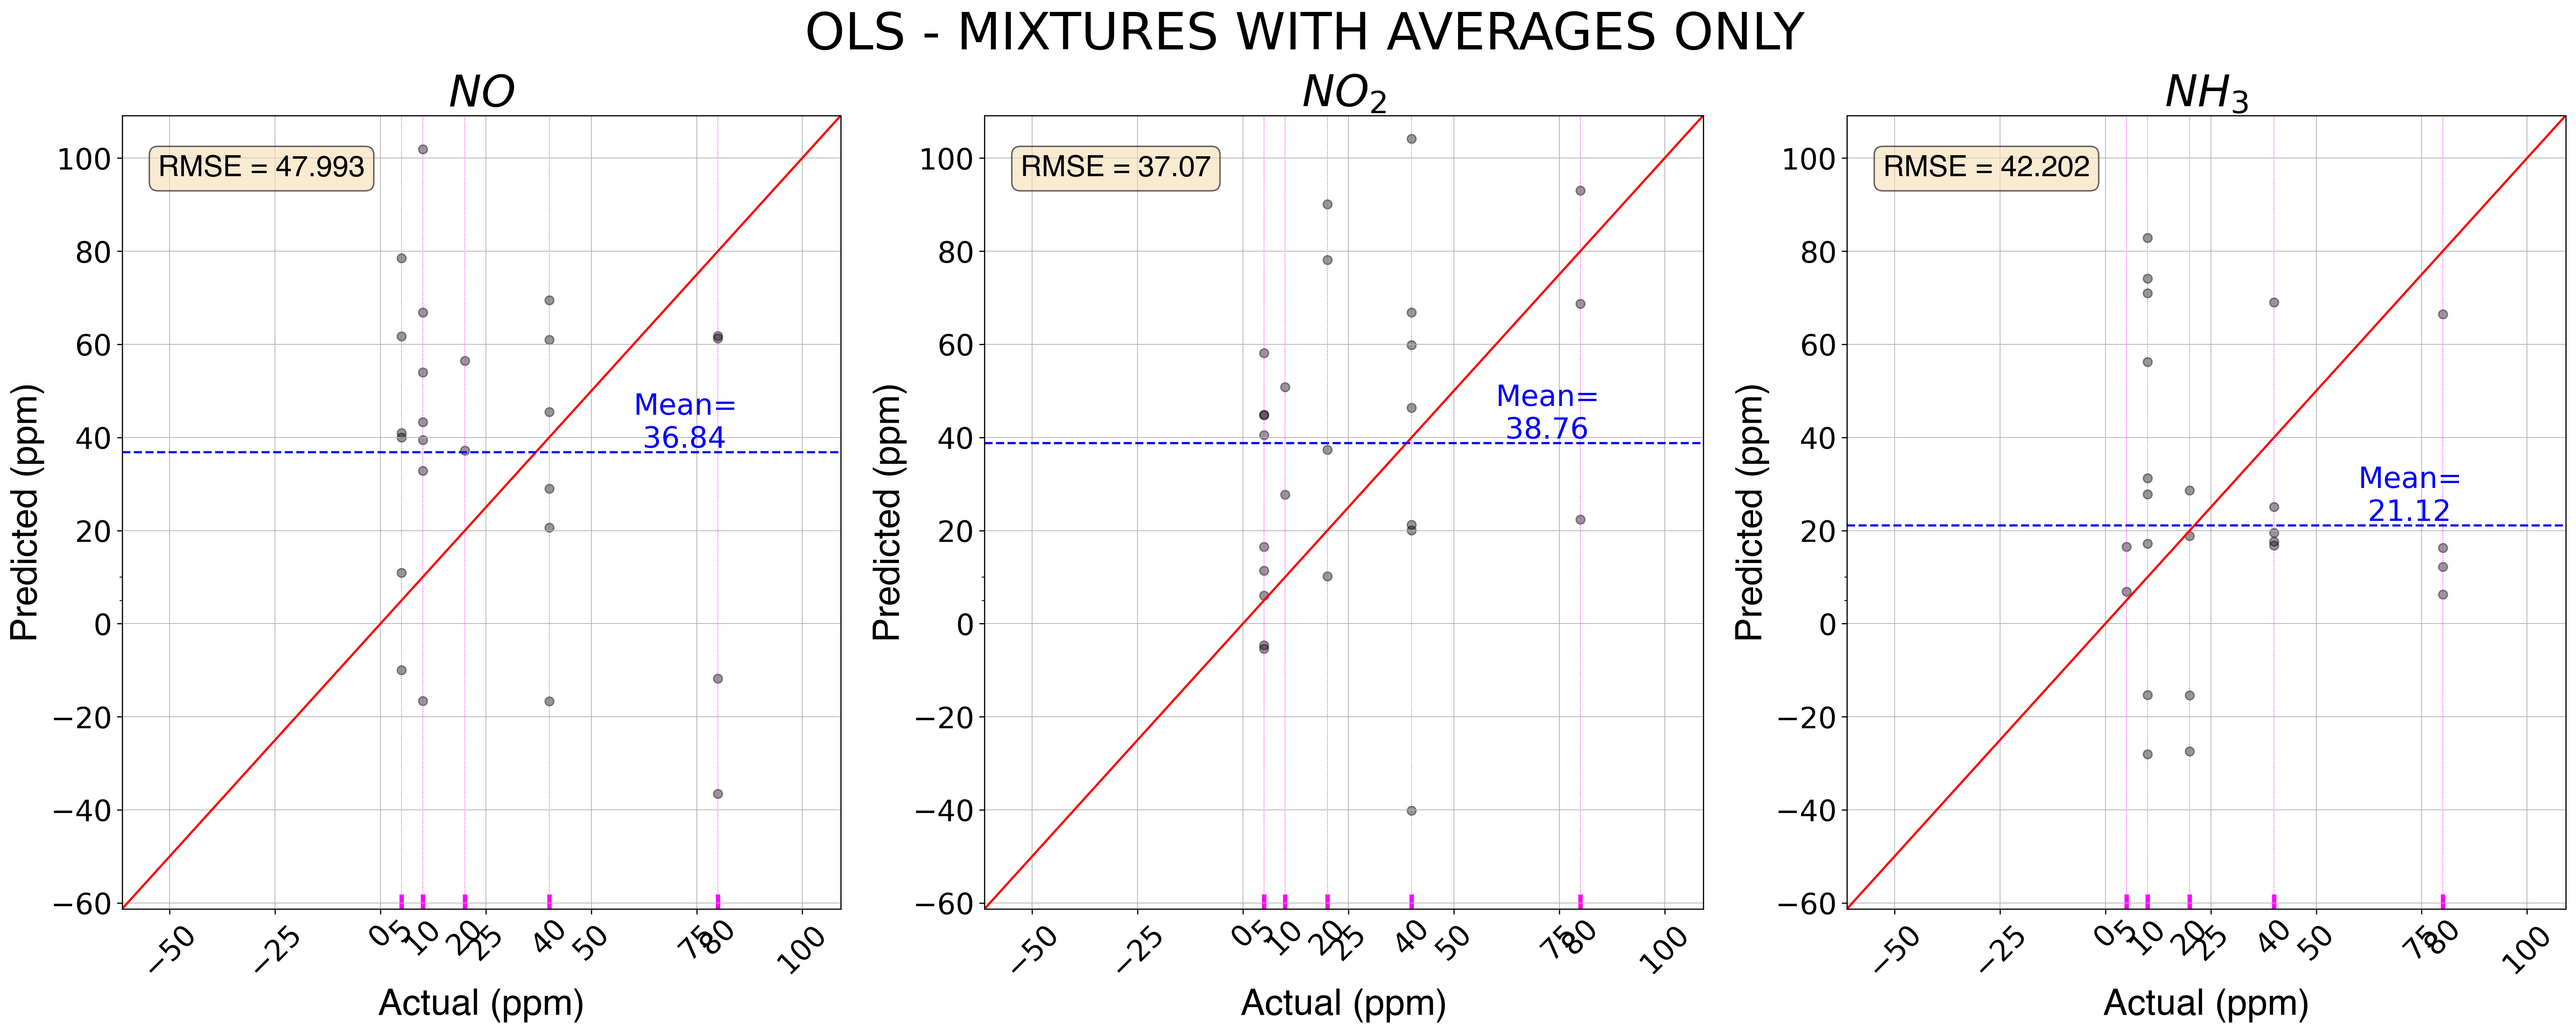
\includegraphics[width=1\linewidth]{../figures/ols-avg-act-vs-pred.png}
		\caption{}
		\label{fig:ols-averaged}
	\end{subfigure}
	
	\caption{Actual vs. Predicted for (a) slopes and averages through exposures and (b) only averaged average features through mixtures.}
	\label{fig:ols-both}
\end{figure}

Each subplot  in Figure~\ref{fig:ols-both} corresponds to predictions of \nox and ammonia concentrations, respectively. The red diagonal line is the $y = f(x) = x$ identity line. The blue line is the mean of predicted concentrations. The text box contains more information regarding the model fit.
\label{fig:OLS-ACTUAL-VS-PRED}

\clearpage
\section{\acrlong{pcr}}
\label{sec:results-pcr}

Following the methodology of Chapter~\ref{cha:methods}, a \acrshort{pca} is conducted with two components in an attempt to visualize the data in a lower dimensional space in Figure~\ref{fig:pca-2components}. 

\begin{figure}[!htb]
	\centering
	
	\begin{subfigure}[b]{1\textwidth}
	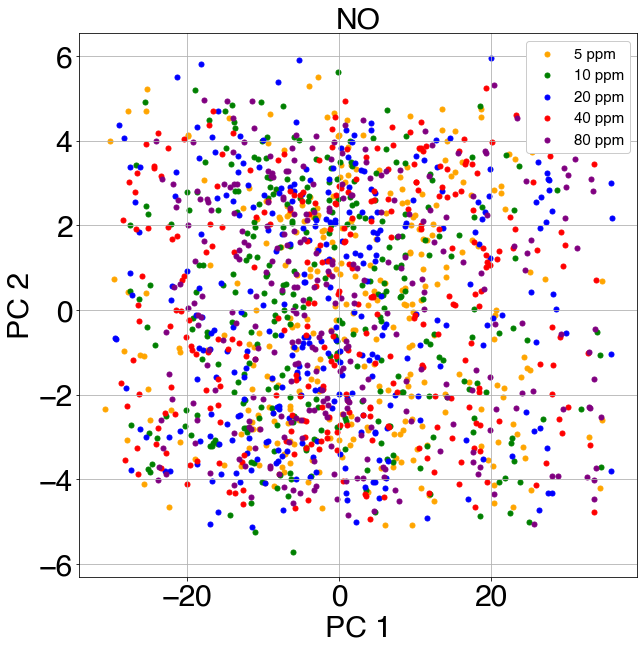
\includegraphics[width=0.30\textwidth]{../../figures/pcaNO.png}
	\hfill
	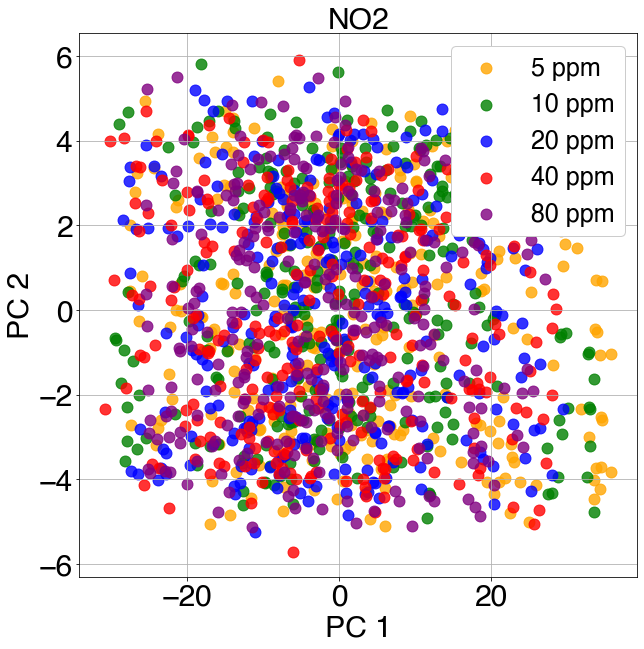
\includegraphics[width=0.30\textwidth]{../../figures/pcaNO2.png}
	\hfill
	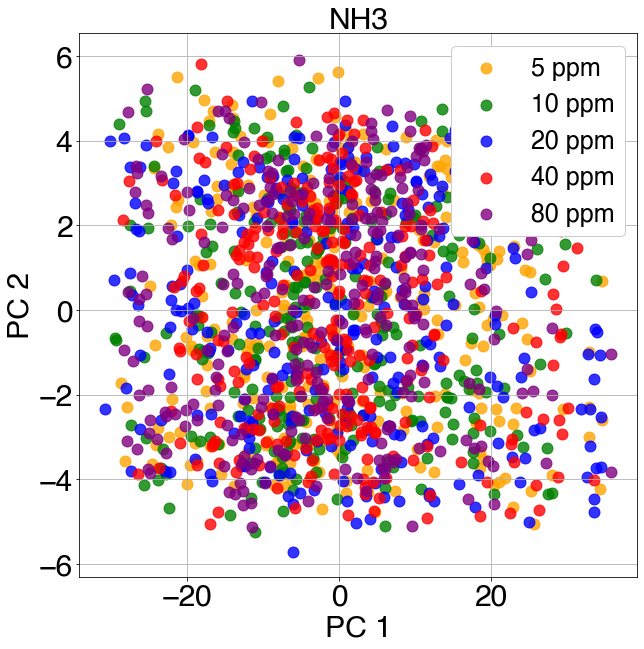
\includegraphics[width=0.30\textwidth]{../../figures/pcaNH3.png}
	\caption{}
	\label{fig:pca}
	\end{subfigure}
	
	\begin{subfigure}[b]{1\textwidth}
	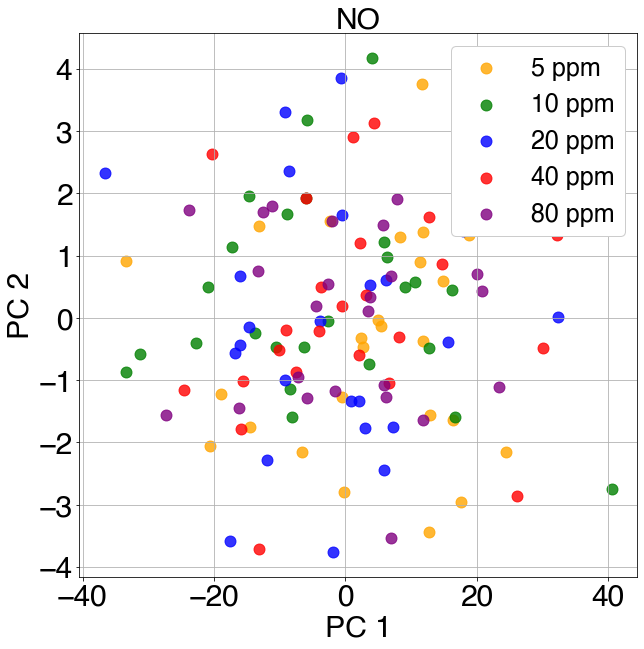
\includegraphics[width=0.30\textwidth]{../../figures/pcaNO-avg-feat.png}
	\hfill
	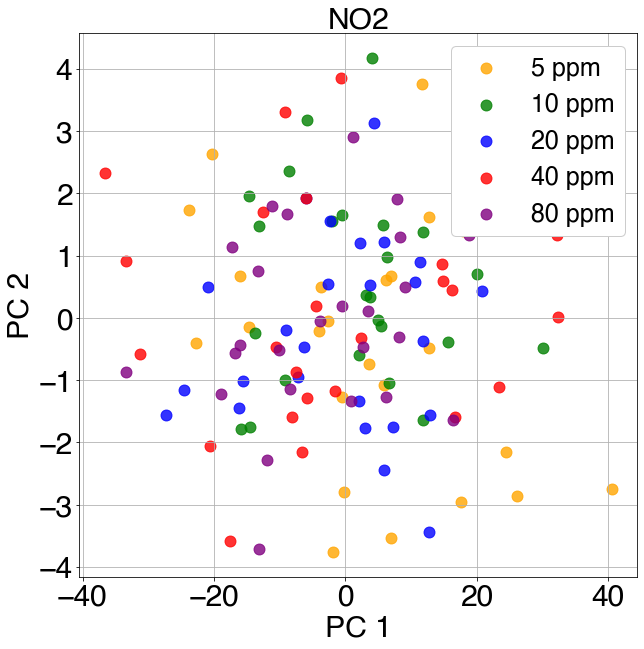
\includegraphics[width=0.30\textwidth]{../../figures/pcaNO2-avg-feat.png}
	\hfill
	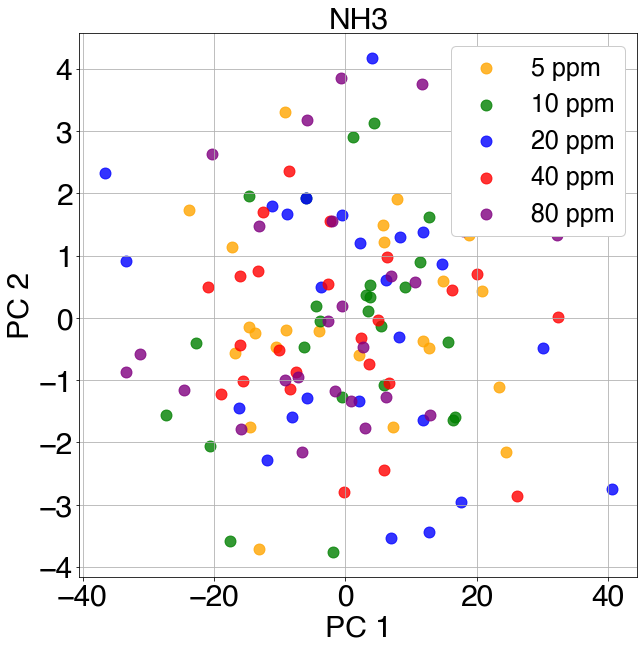
\includegraphics[width=0.30\textwidth]{../../figures/pcaNH3-avg-feat.png}
	\caption{}
	\label{fig:pca-avg-only}
	\end{subfigure}
	
	\caption{\acrshort{pca} for (a) slopes and averages through exposures and (b) only averaged average features through mixtures.}
	\label{fig:pca-both}
\end{figure}

Furthermore, an explained variance plot is shown in Figure~\ref{fig:pcr-exp-var-both}. For the first case, the first two \acrshort{pc}s explain approximately 40\% of the total variance, reaching 80\% around 100 components. On the other hand, the second case achieves 90\% of explained variability with two components.

\begin{figure}[!htb]
	\centering

	\begin{subfigure}[t]{0.5\textwidth}
		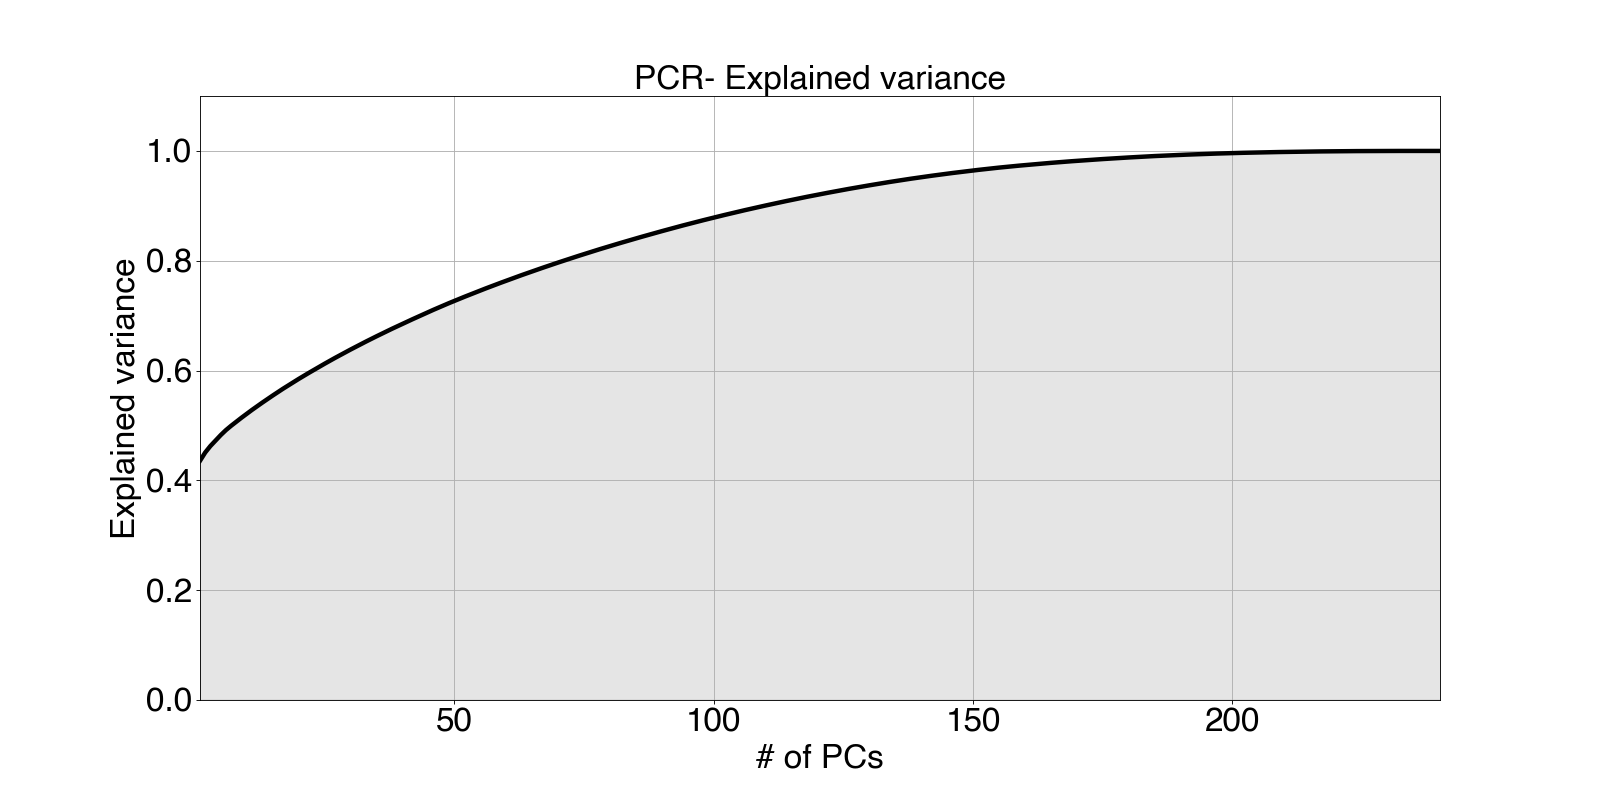
\includegraphics[width=1\linewidth]{../figures/pcr-explained-variance.png}
		\caption{}
		\label{fig:pca-exp-var} 
	\end{subfigure}
	
	\begin{subfigure}[t]{0.5\textwidth}
		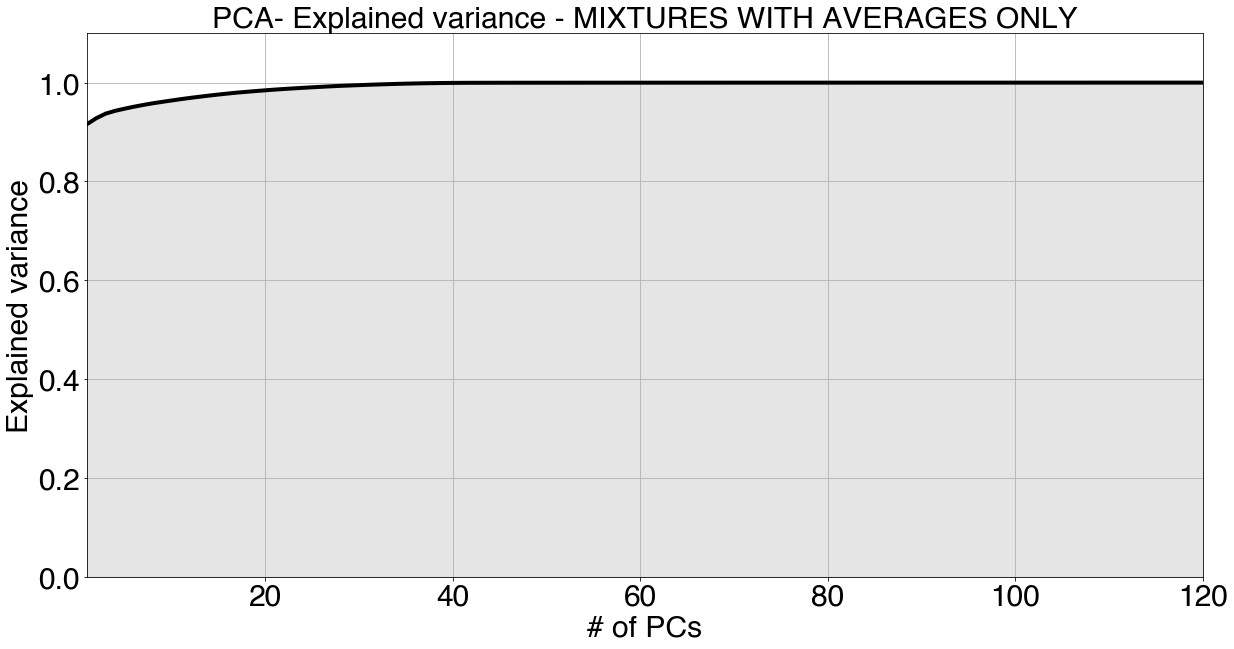
\includegraphics[width=1\linewidth]{../figures/pcr-explained-variance-avg-feat.png}
		\caption{}
		\label{fig:pca-exp-var-averaged}
	\end{subfigure}
	
	\caption{Explained variance of \acrshort{pc} for (a) slopes and averages through exposures and (b) only averaged average features through mixtures.}
	\label{fig:pca-exp-var-both}
\end{figure}

After this exploration of \acrshort{pca}, the analysis proceeds to fit a \acrshort{pcr} model to the data. The choice of number of \acrshort{pc}s was made via cross-validation using \acrshort{rmse} as the loss function, as can be seen in Figure~\ref{fig:pcr-cv-both}. Choosing only one components yields the minimum loss for both cases, around 27.

\begin{figure}[!htb]
	\centering
	
	\begin{subfigure}[t]{0.5\textwidth}
		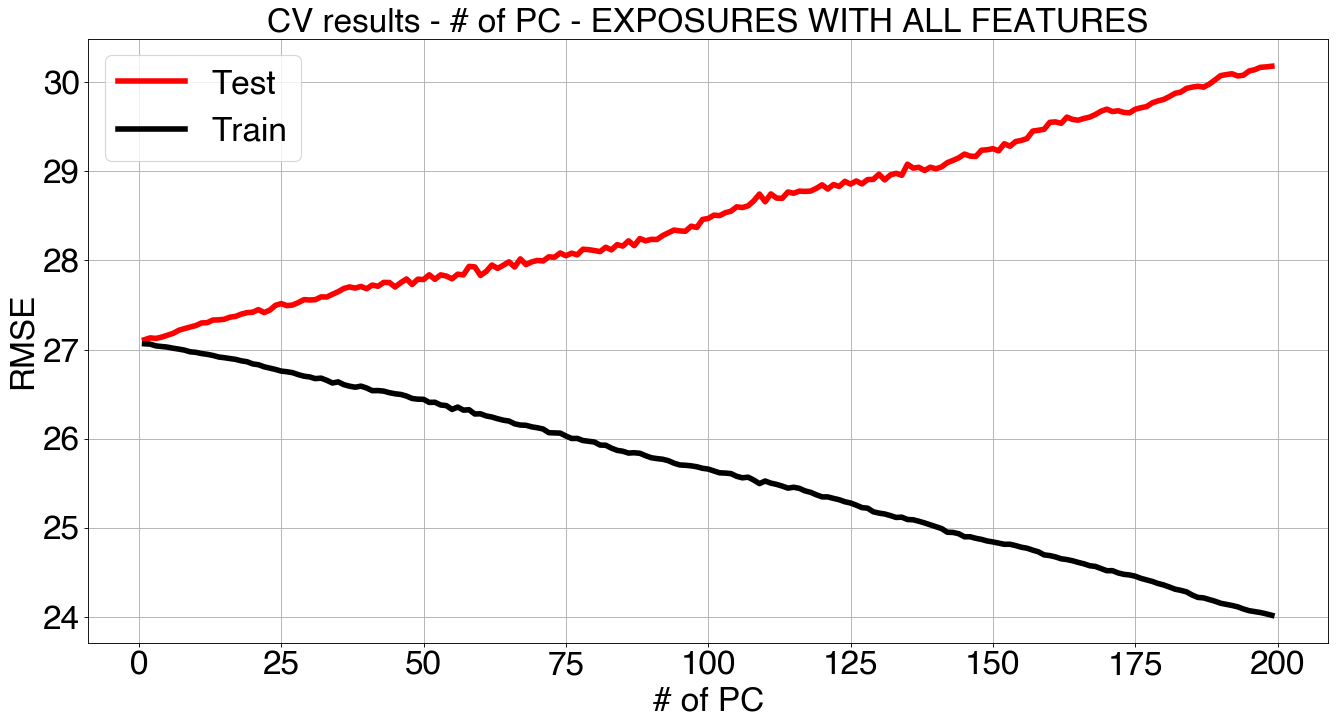
\includegraphics[width=1\linewidth]{../figures/pcr-cv.png}
		\caption{}
		\label{fig:pcr-cv} 
	\end{subfigure}
	
	\begin{subfigure}[t]{0.5\textwidth}
		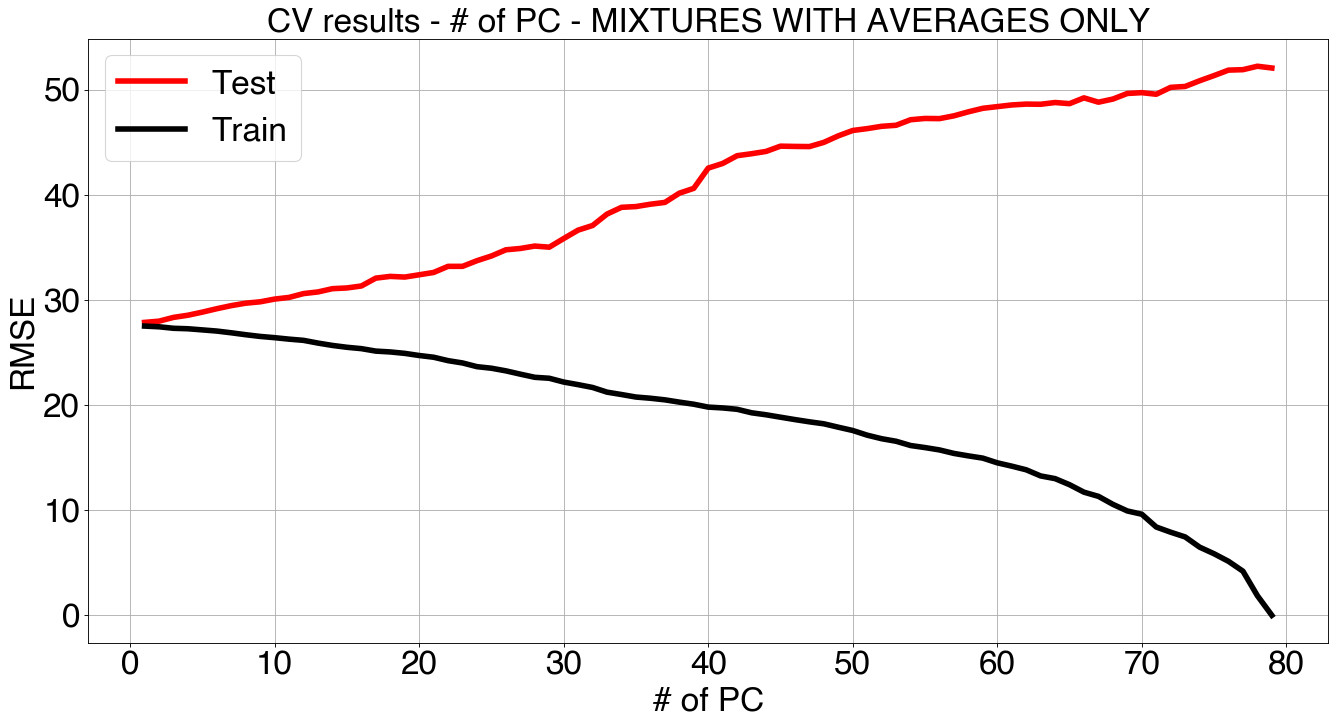
\includegraphics[width=1\linewidth]{../figures/pcr-cv-avg-feat.png}
		\caption{}
		\label{fig:pcr-cv-averaged}
	\end{subfigure}
	
	\caption{Cross-validation results for (a) slopes and averages through exposures and (b) only averaged average features through mixtures.}
	\label{fig:pcr-cv-both}
\end{figure}

After the choosing the number of components, the regression was fit to the training data and used to predict unseen validation data. The results are shown in Figure~\ref{fig:pcr-both}.

\begin{figure}[!htb]
	\centering
	
	\begin{subfigure}[t]{1\textwidth}
		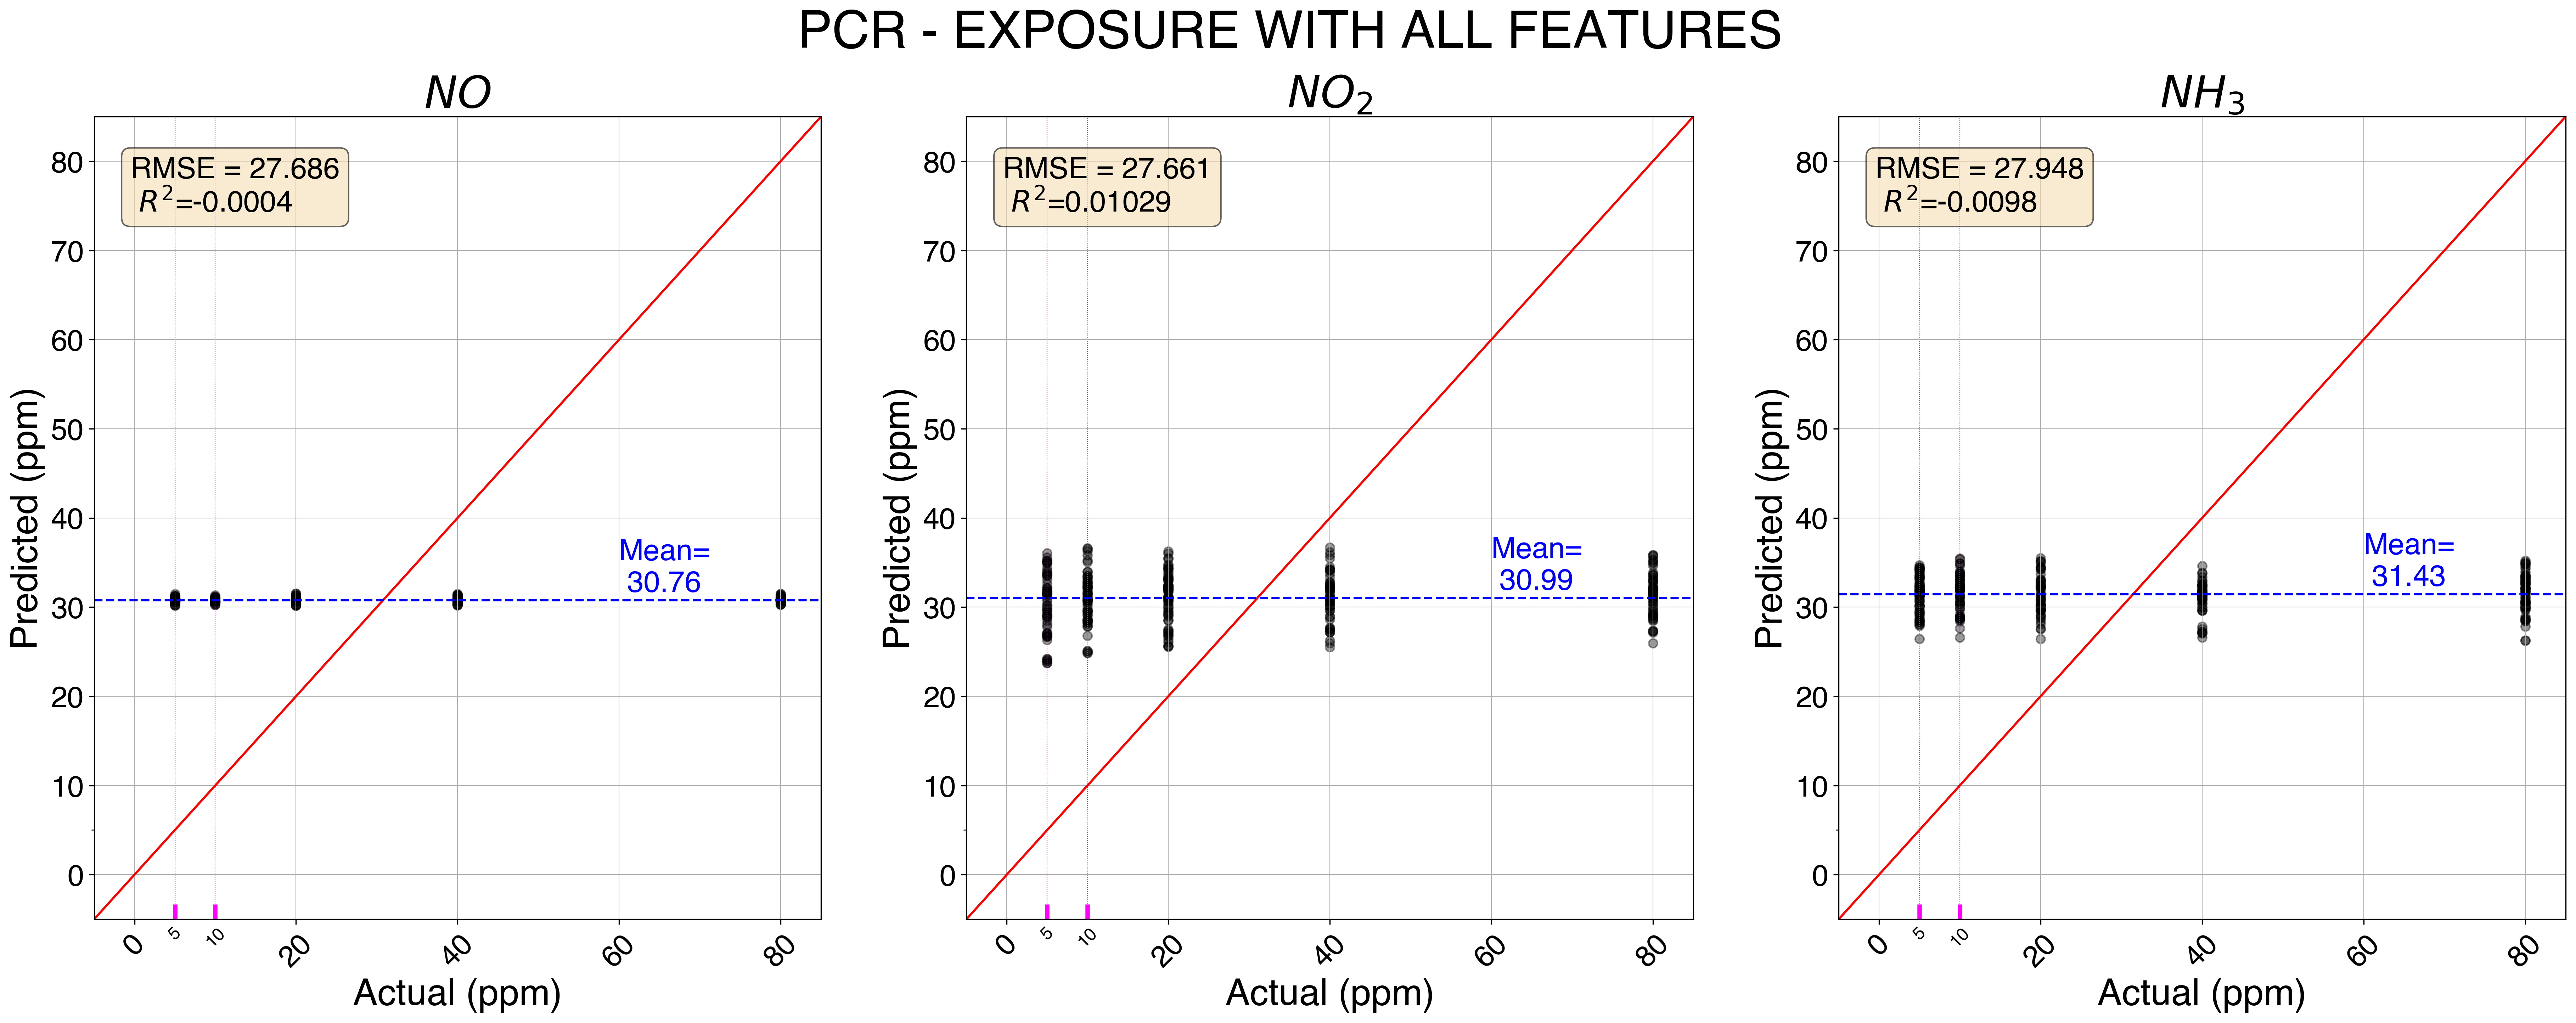
\includegraphics[width=1\linewidth]{../figures/pcr-act-vs-pred.png}
		\caption{}
		\label{fig:pcr-act-vs-pred} 
	\end{subfigure}
	
	\begin{subfigure}[t]{1\textwidth}
		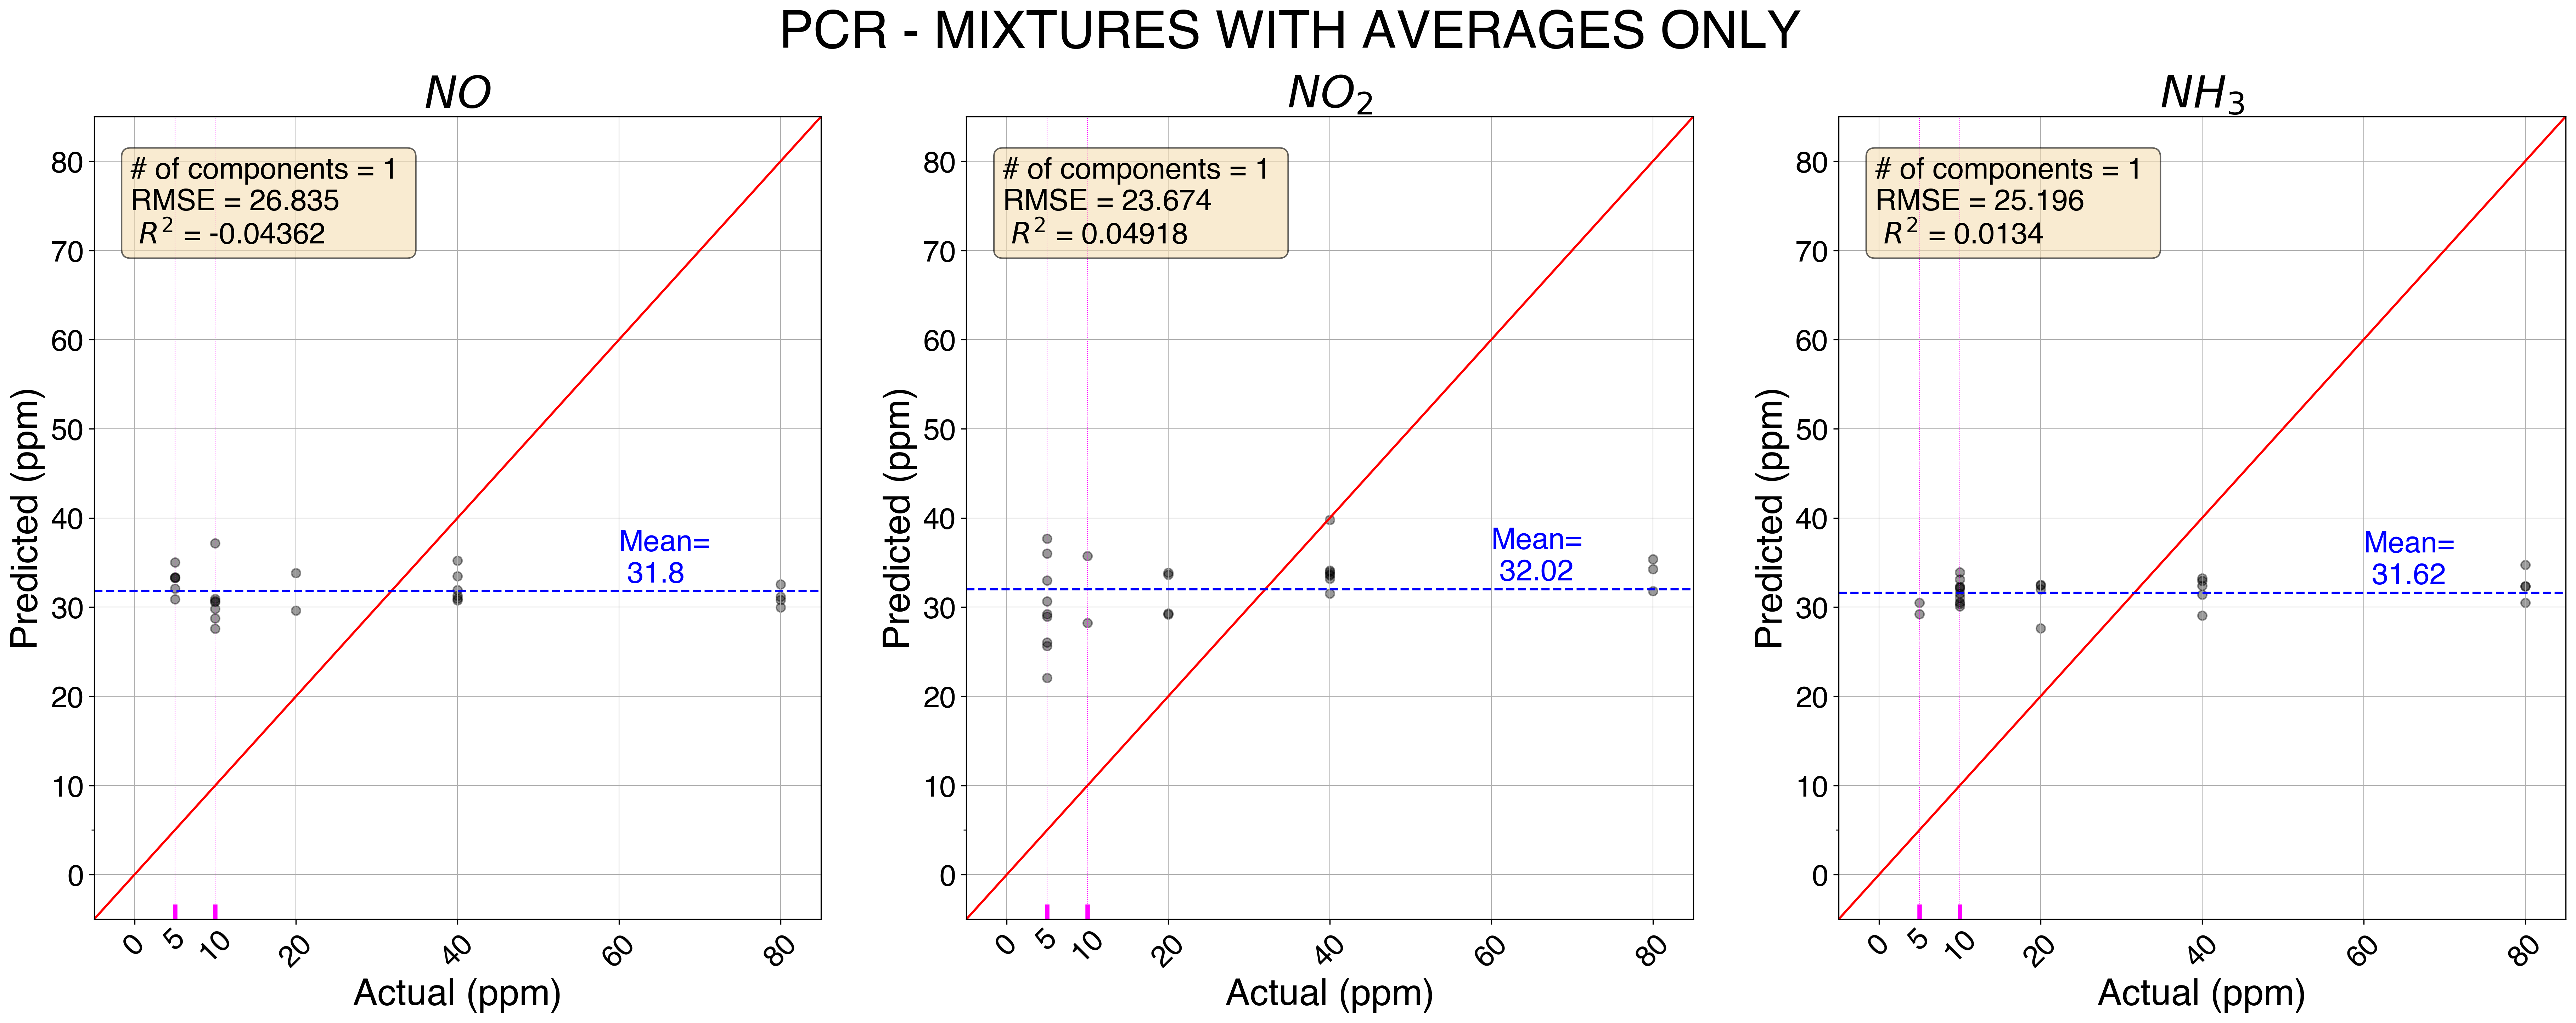
\includegraphics[width=1\linewidth]{../figures/pcr-act-vs-pred-avg-feat.png}
		\caption{}
		\label{fig:pcr-act-vs-pred-avg-feat}
	\end{subfigure}
	
	\caption{\acrshort{pcr} for (a) slopes and averages through exposures and (b) only averaged average features through mixtures.}
	\label{fig:pcr-both}
\end{figure}

\clearpage
\section{\acrlong{plsr}}
\label{sec:results-plsr}

Following the proposed model progression, the analysis proceeds to fit the \acrshort{plsr} model. A similar pipeline to Section~\ref{sec:results-pcr} was used. First, in Figure~\ref{fig:pls-both}, the choice of only two \acrshort{pls} components allowed visualization of data in a two dimensional plot. Moreover, total explained variance is shown in Figure~\ref{fig:pls-exp-var-both}. Once again, cross-validation using \acrshort{rmse} yields a single component as the best choice, which is then used to fit and predict gas concentrations in Figure~\ref{fig:plsr-actual-vs-pred-both}.

\begin{figure}[!htb]
	\centering
	
	\begin{subfigure}[b]{1\textwidth}
		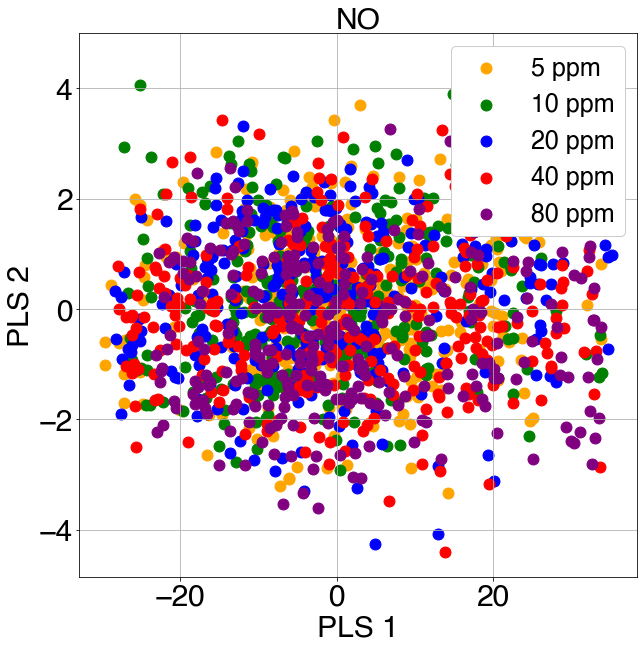
\includegraphics[width=0.30\textwidth]{../../figures/plsNO.png}
		\hfill
		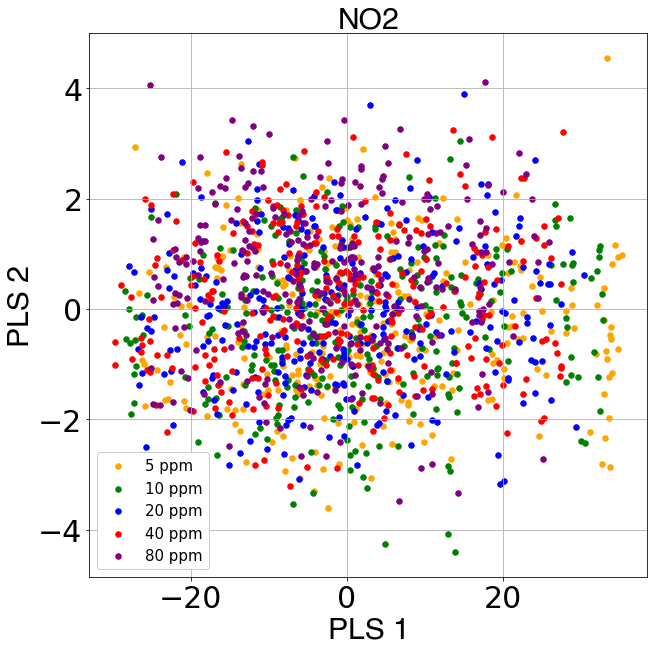
\includegraphics[width=0.30\textwidth]{../../figures/plsNO2.png}
		\hfill
		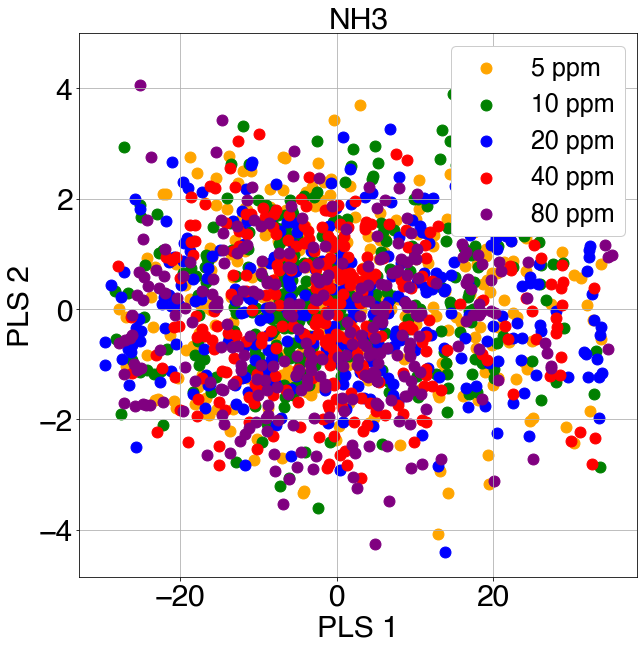
\includegraphics[width=0.30\textwidth]{../../figures/plsNH3.png}
		\caption{}
		\label{fig:pls}
	\end{subfigure}
	
	\begin{subfigure}[b]{1\textwidth}
		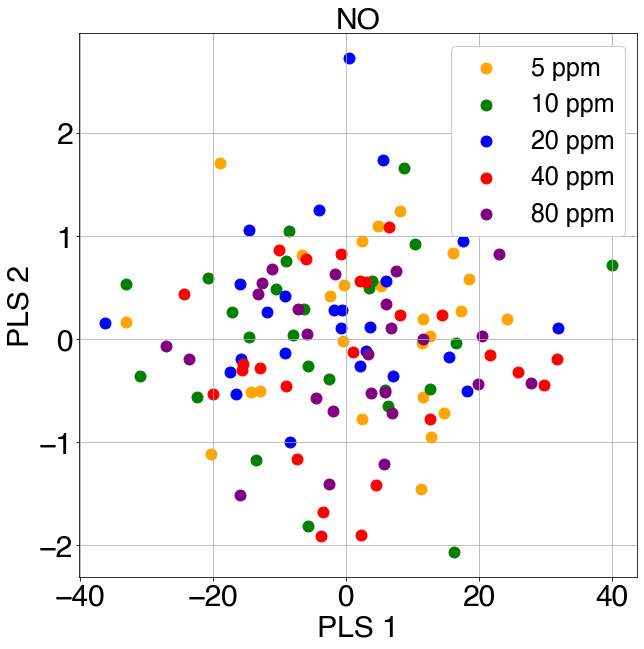
\includegraphics[width=0.30\textwidth]{../../figures/plsNO-avg-feat.png}
		\hfill
		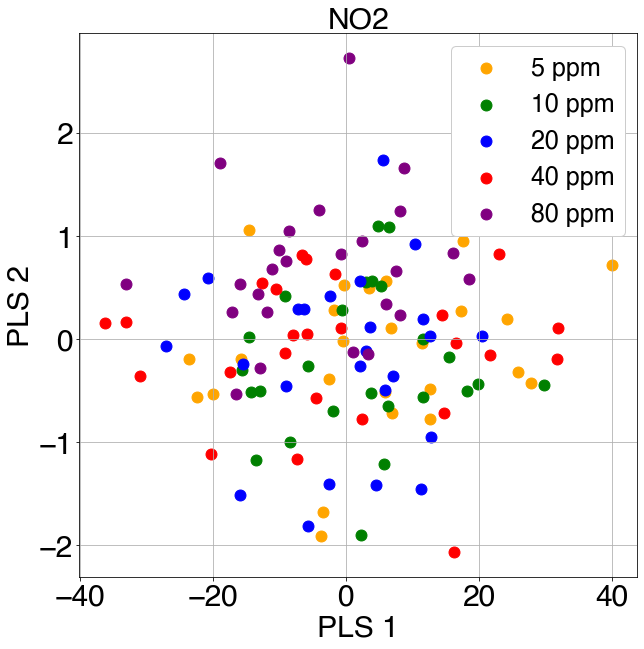
\includegraphics[width=0.30\textwidth]{../../figures/plsNO2-avg-feat.png}
		\hfill
		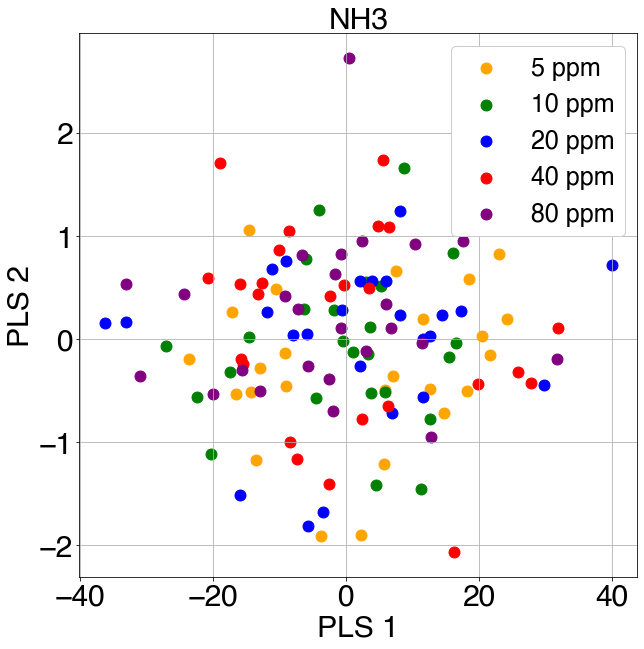
\includegraphics[width=0.30\textwidth]{../../figures/plsNH3-avg-feat.png}
		\caption{}
		\label{fig:pls-avg-only}
	\end{subfigure}
	
	\caption{\acrshort{pls} scores for (a) slopes and averages through exposures and (b) only averaged average features through mixtures.}
	\label{fig:pls-both}
\end{figure}

\begin{figure}[!htb]
	\centering
	
	\begin{subfigure}[t]{0.5\textwidth}
		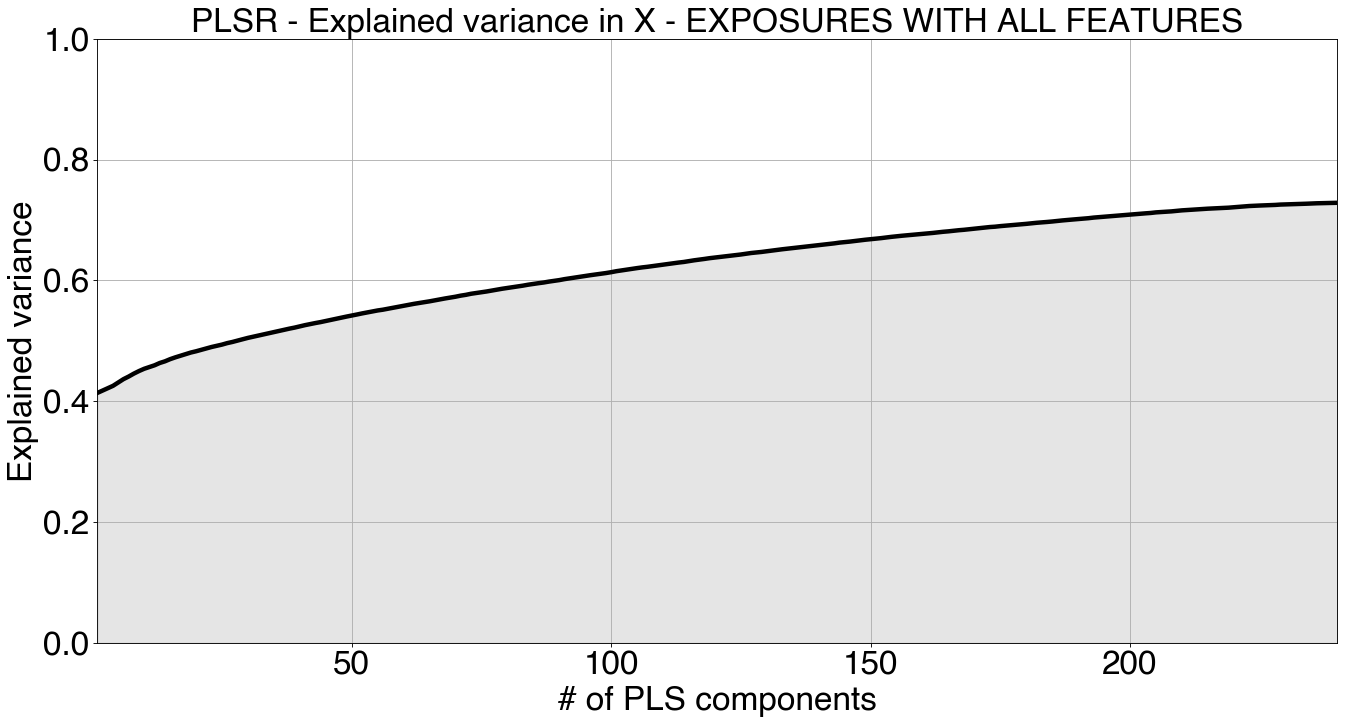
\includegraphics[width=1\linewidth]{../figures/pls-explained-variance.png}
		\caption{}
		\label{fig:pls-exp-var} 
	\end{subfigure}
	
	\begin{subfigure}[t]{0.5\textwidth}
		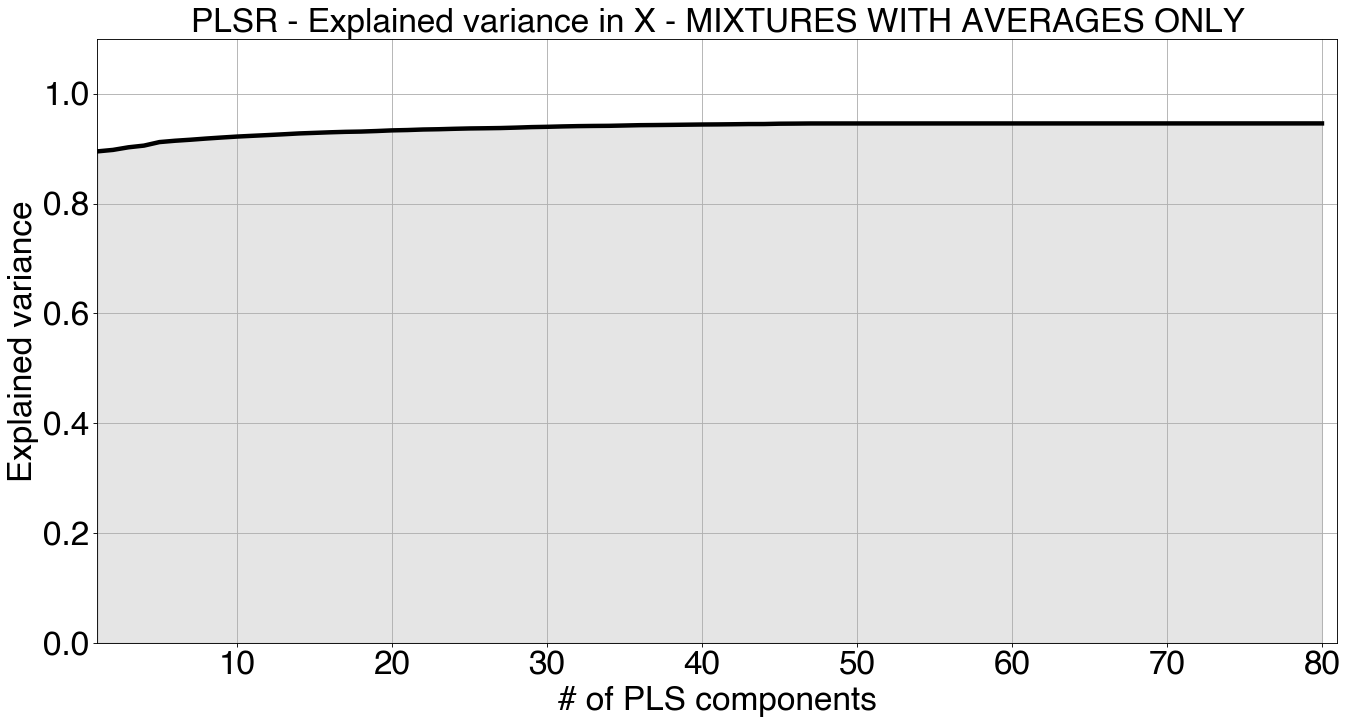
\includegraphics[width=1\linewidth]{../figures/pls-explained-variance-avg-feat.png}
		\caption{}
		\label{fig:pls-exp-var-avg-feat}
	\end{subfigure}
	
	\caption{Explained variance of \acrshort{pls} components for (a) slopes and averages through exposures and (b) only averaged average features through mixtures.}
	\label{fig:pls-exp-var-both}
\end{figure}


\begin{figure}[!htb]
	\centering
	
	\begin{subfigure}[t]{0.5\textwidth}
		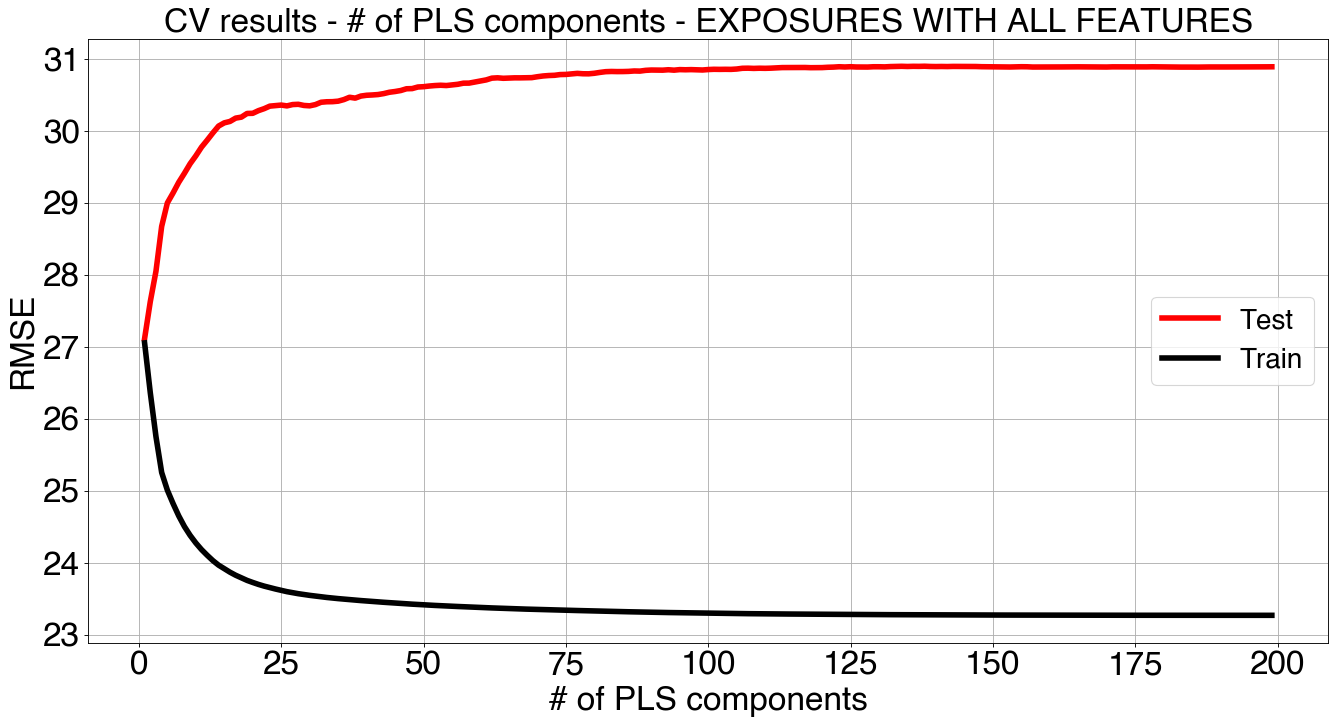
\includegraphics[width=1\linewidth]{../figures/pls-cv.png}
		\caption{}
		\label{fig:pls-cv} 
	\end{subfigure}
	
	\begin{subfigure}[t]{0.5\textwidth}
		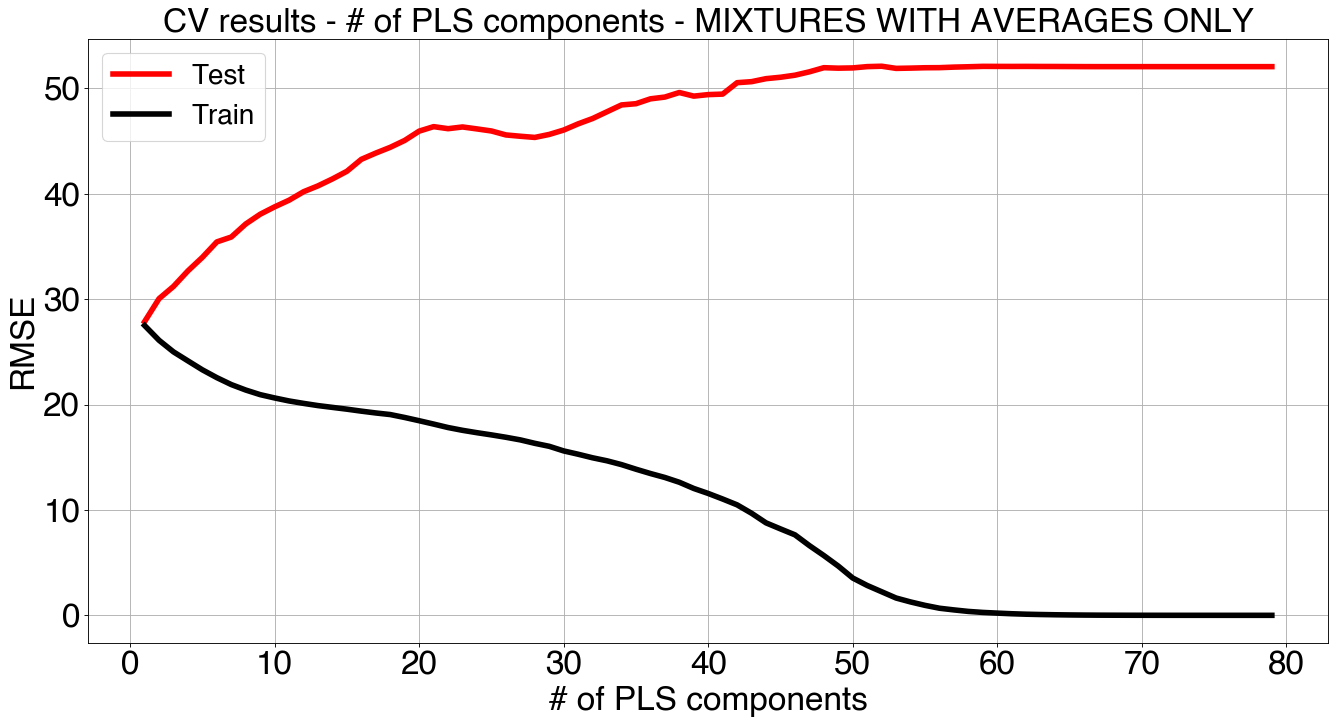
\includegraphics[width=1\linewidth]{../figures/pls-cv-avg-feat.png}
		\caption{}
		\label{fig:pls-cv-avg-feat}
	\end{subfigure}
	
	\caption{Cross-validation results for (a) slopes and averages through exposures and (b) only averaged average features through mixtures.}
	\label{fig:pls-cv-both}
\end{figure}

\begin{figure}[!htb]
	\centering
	
	\begin{subfigure}[t]{1\textwidth}
		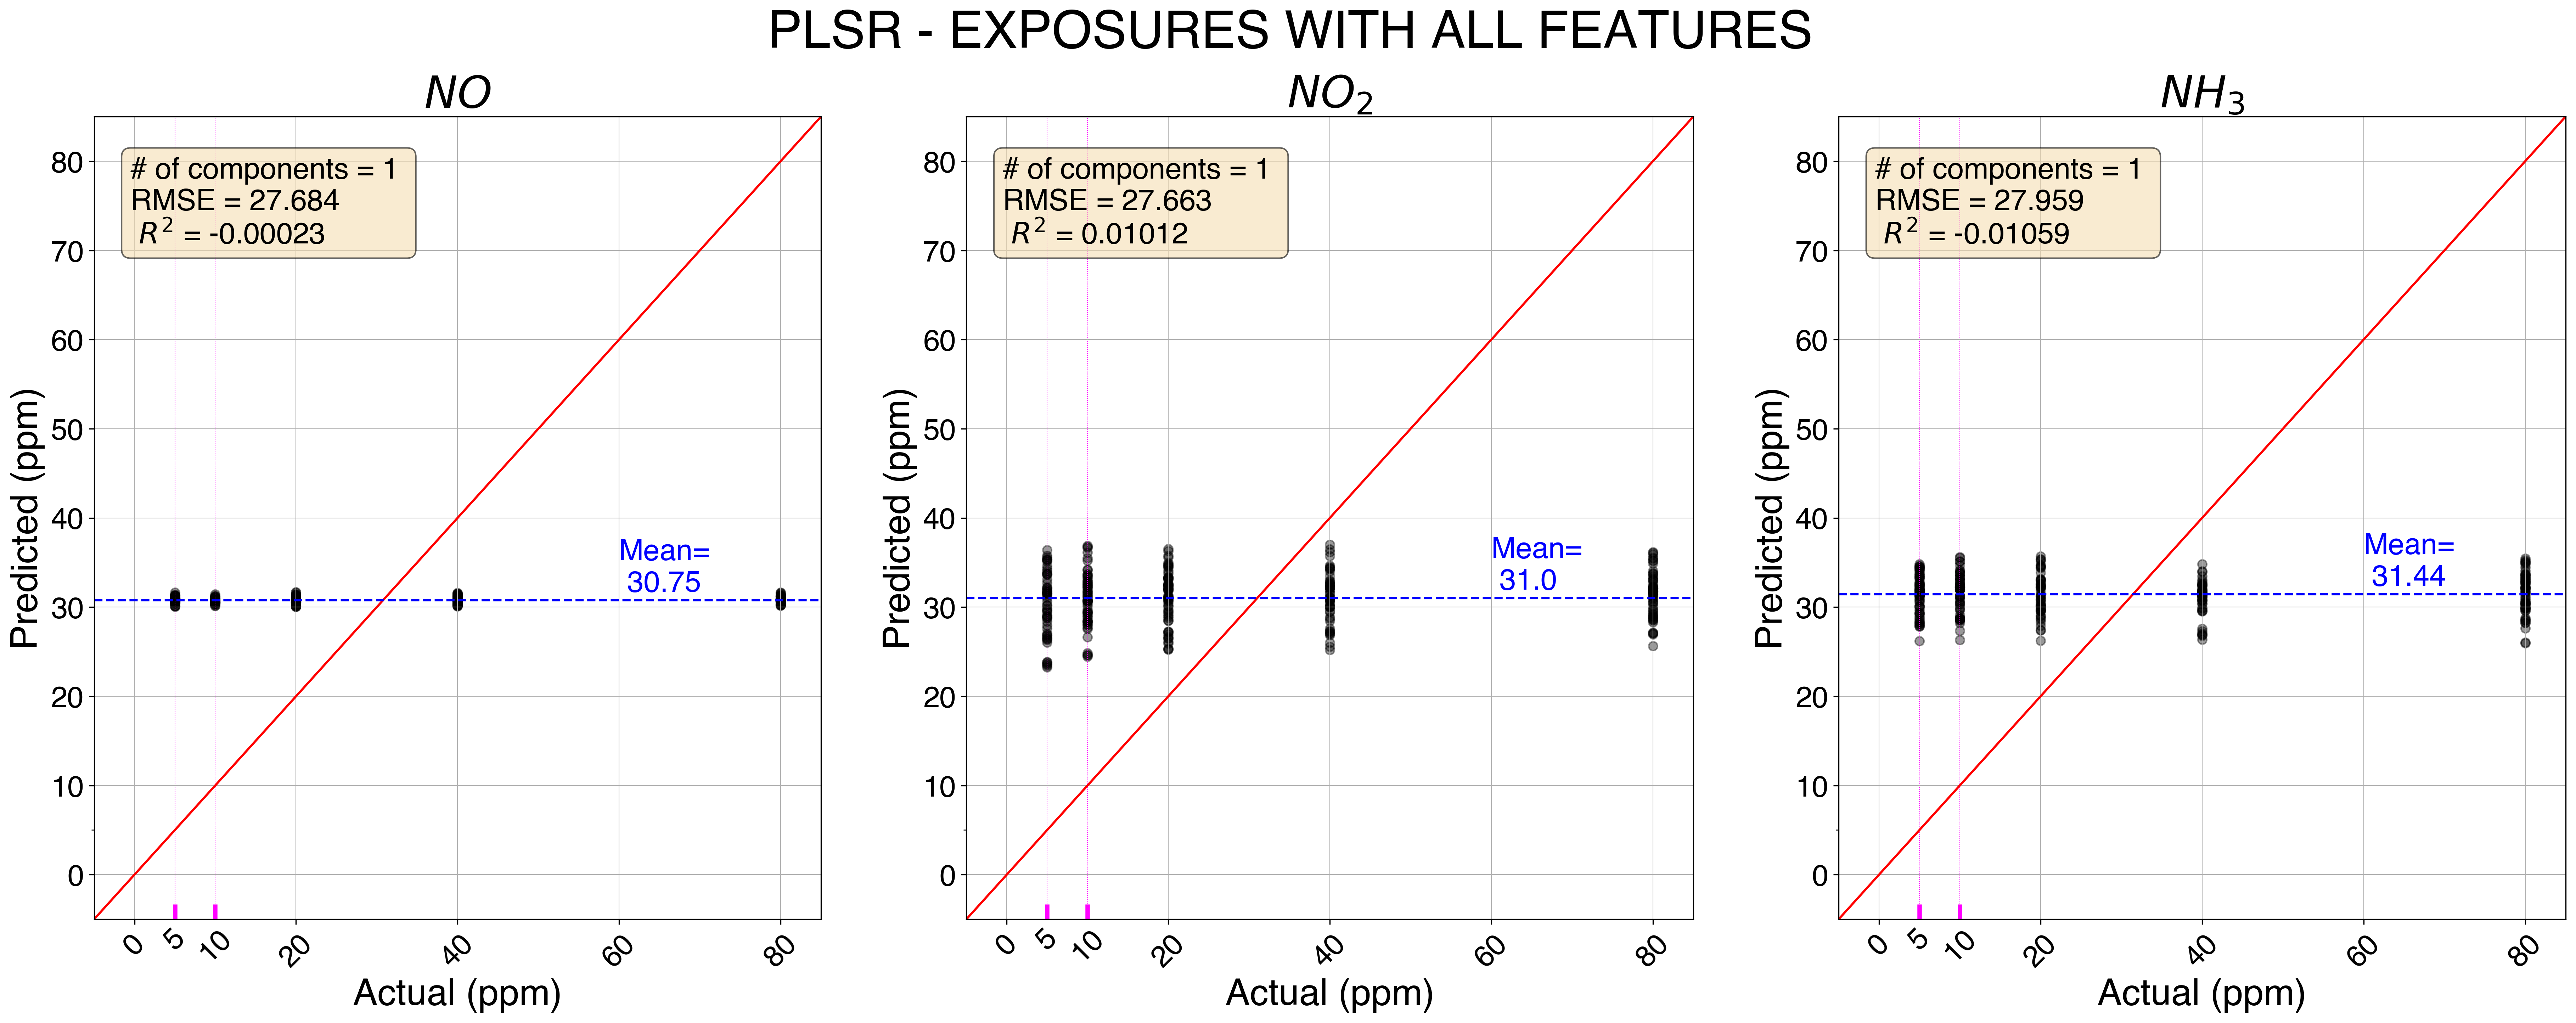
\includegraphics[width=1\linewidth]{../figures/plsr-act-vs-pred.png}
		\caption{}
		\label{fig:pls-act-vs-pred} 
	\end{subfigure}
	
	\begin{subfigure}[t]{1\textwidth}
		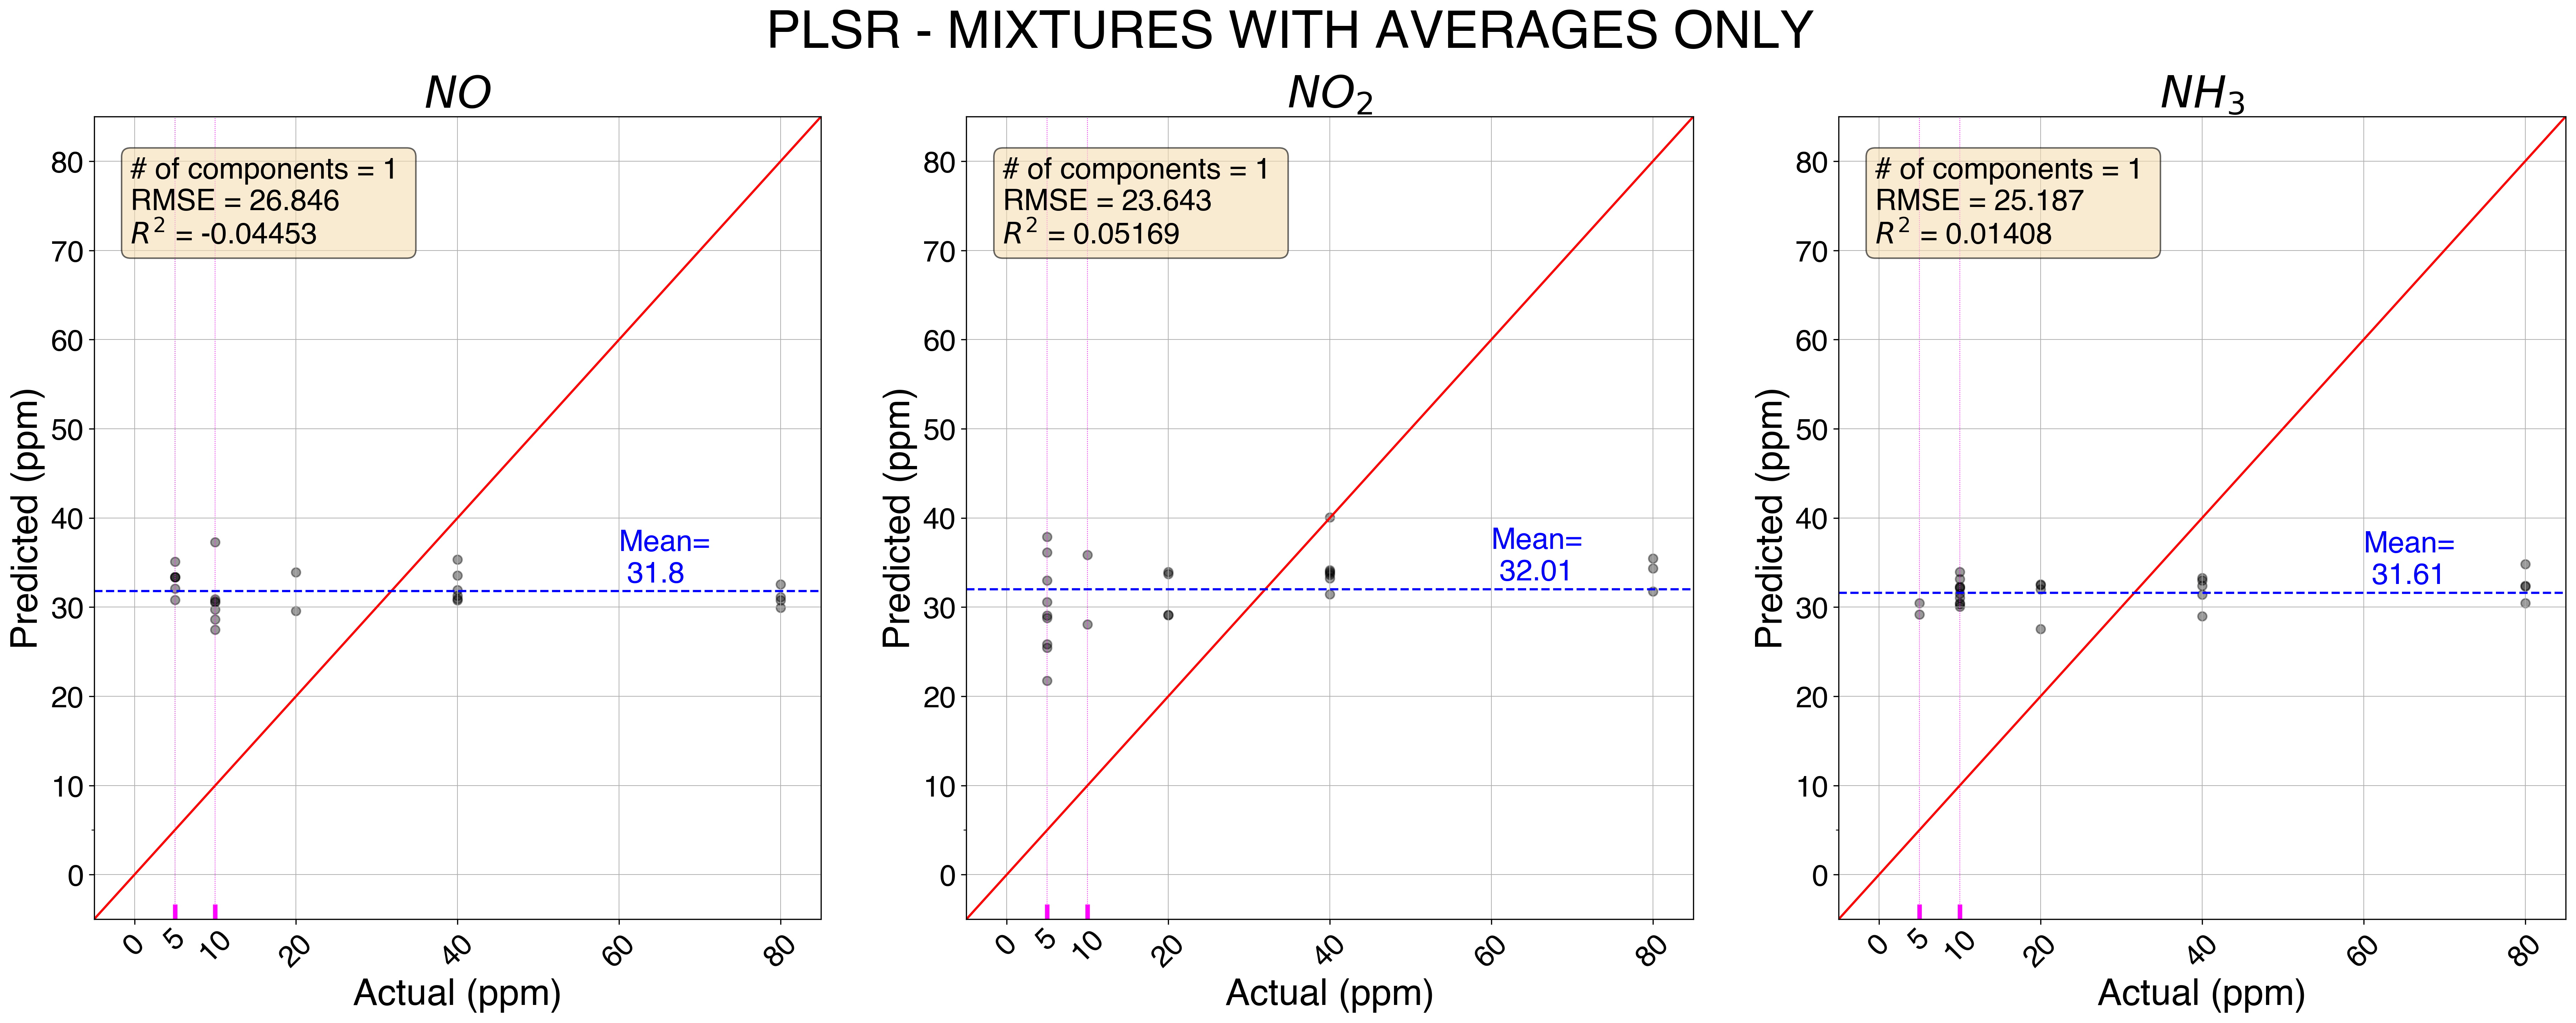
\includegraphics[width=1\linewidth]{../figures/plsr-act-vs-pred-avg-feat.png}
		\caption{}
		\label{fig:pls-act-vs-pred-avg-feat}
	\end{subfigure}
	
	\caption{\acrshort{plsr} for (a) slopes and averages through exposures and (b) only averaged average features through mixtures.}
	\label{fig:plsr-actual-vs-pred-both}
\end{figure}

\clearpage
\section{Ridge Regression}
\label{sec:results-ridge}

For Ridge regression, the regularization term $\lambda$ was chosen via cross-validation, as shown in Figure~\ref{fig:ridge-cv-both}. Additionally, the shrinkage of coefficients can be seen in Figure~\ref{fig:ridge-shrink-both}. As expected, the coefficients shrink asymptotically towards zero.

\begin{figure}[!htb]
	\centering
	
	\begin{subfigure}[t]{0.6\textwidth}
		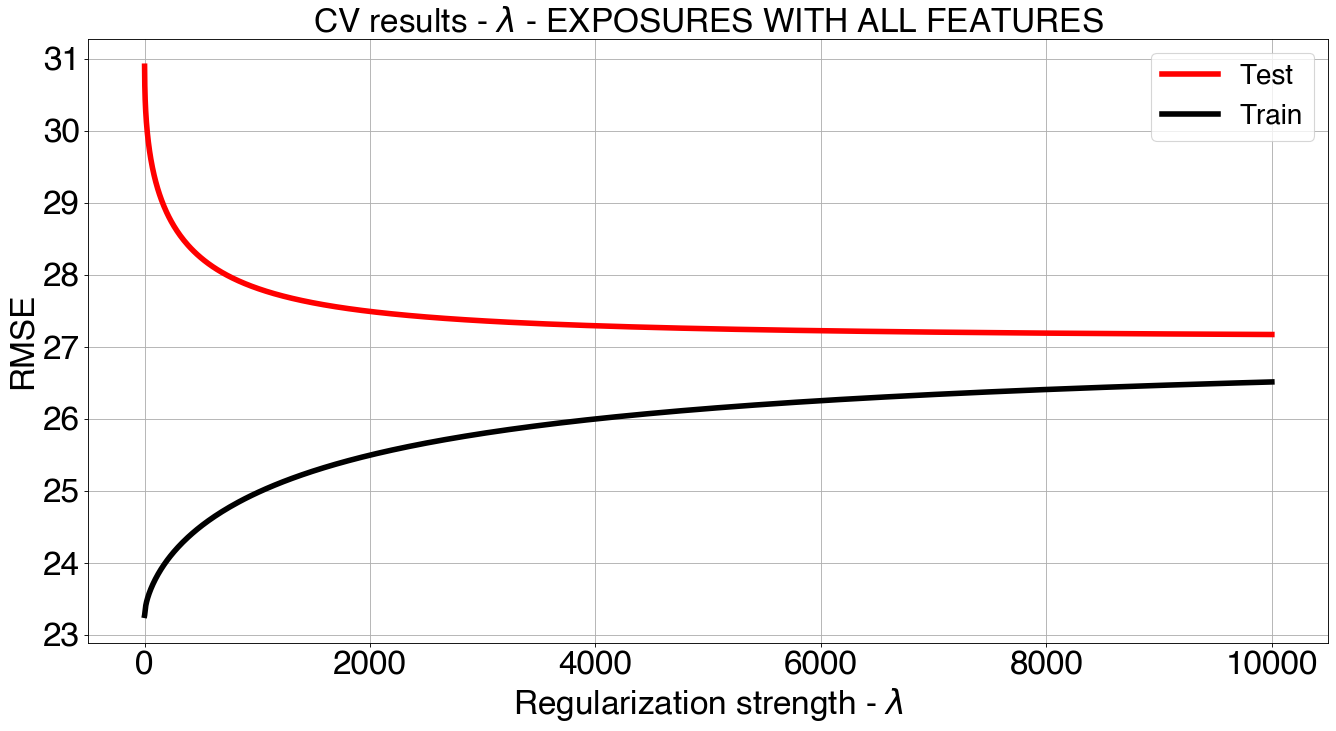
\includegraphics[width=1\linewidth]{../figures/ridge-cv.png}
		\caption{}
		\label{ridge:pls-cv} 
	\end{subfigure}
	
	\begin{subfigure}[t]{0.6\textwidth}
		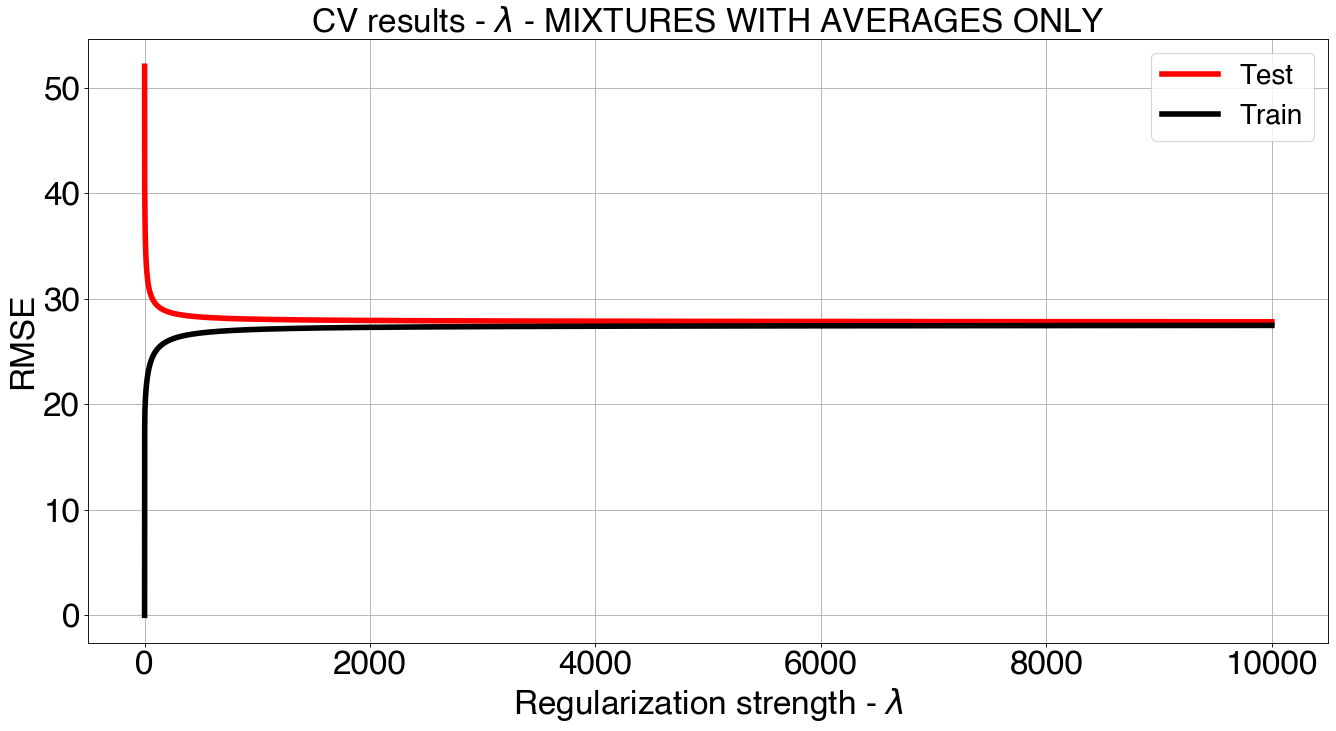
\includegraphics[width=1\linewidth]{../figures/ridge-cv-avg-feat.png}
		\caption{}
		\label{fig:ridge-cv-avg-feat}
	\end{subfigure}
	
	\caption{Cross-validation results for (a) slopes and averages through exposures and (b) only averaged average features through mixtures.}
	\label{fig:ridge-cv-both}
\end{figure}

\begin{figure}[!htb]
	\centering
	
	\begin{subfigure}[t]{0.6\textwidth}
		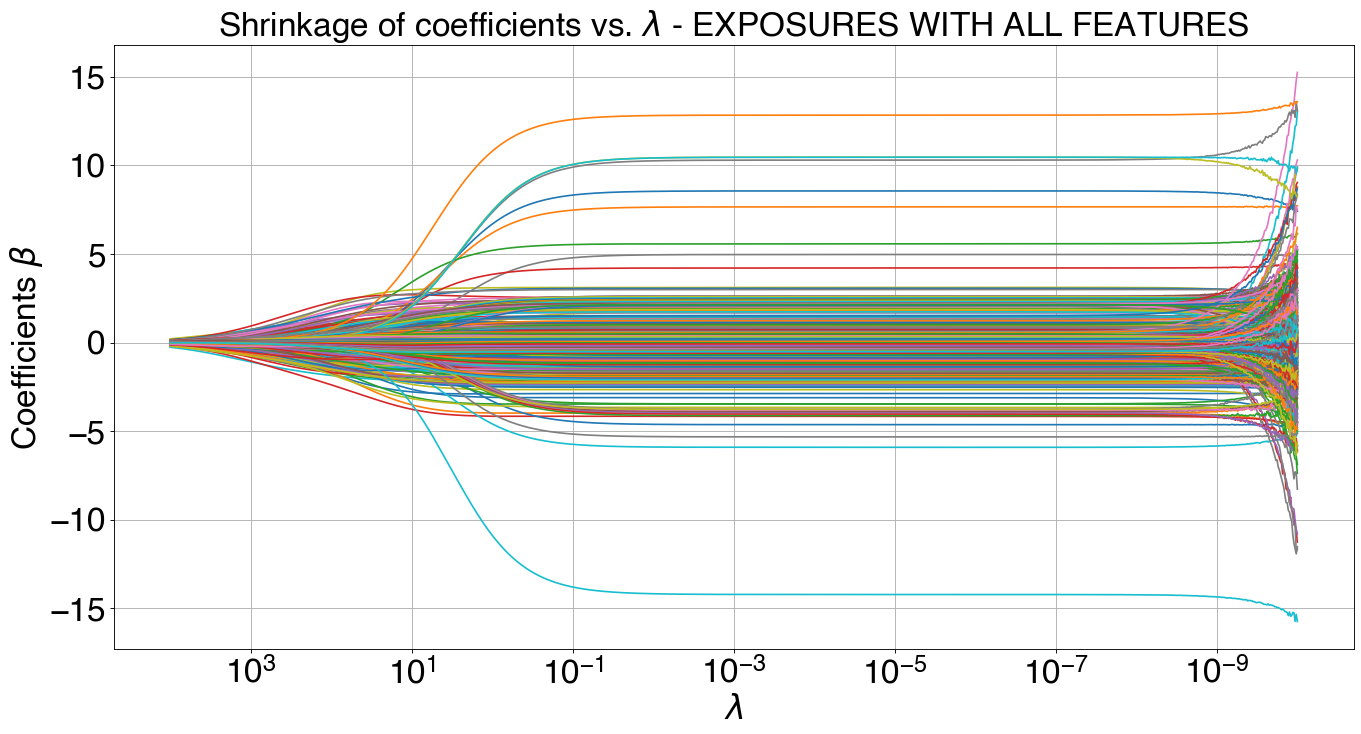
\includegraphics[width=1\linewidth]{../figures/ridge-shrink.png}
		\caption{}
		\label{fig:ridge-shrink} 
	\end{subfigure}
	
	\begin{subfigure}[t]{0.6\textwidth}
		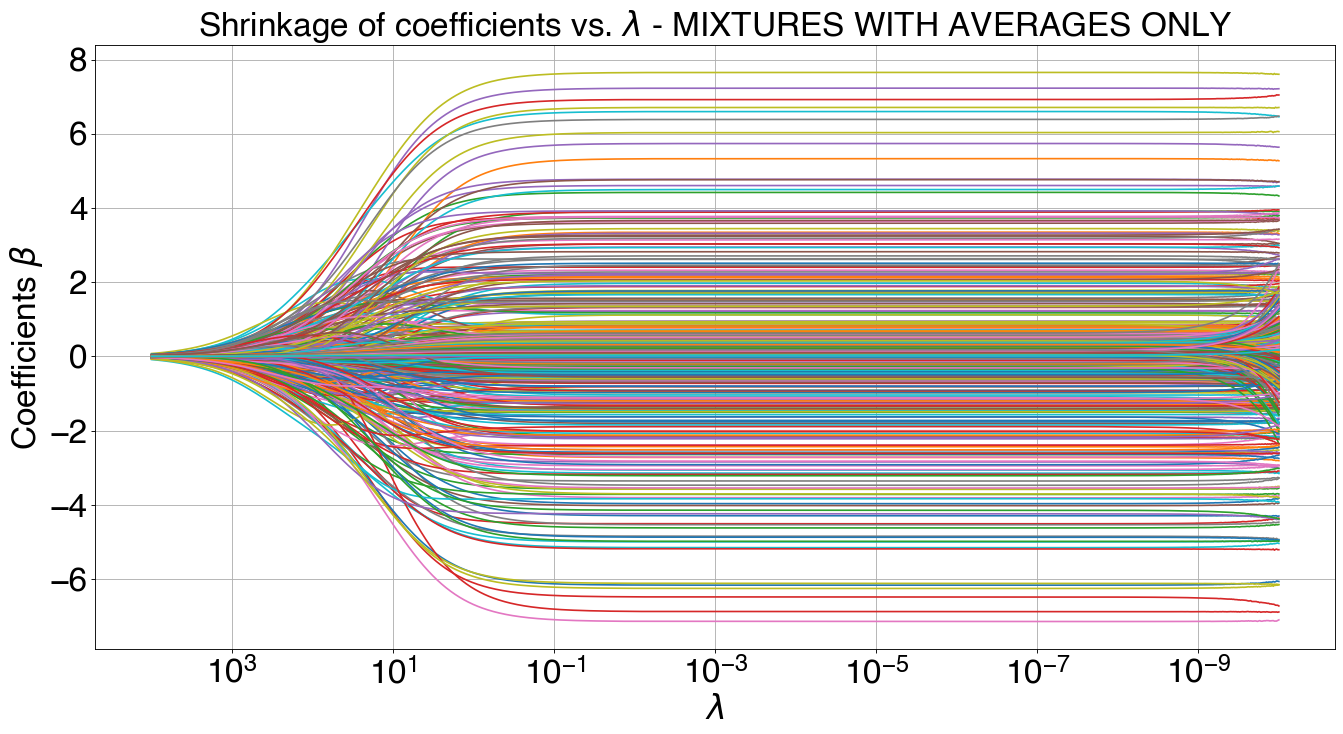
\includegraphics[width=1\linewidth]{../figures/ridge-shrink-avg-feat.png}
		\caption{}
		\label{fig:ridge-shrink-avg-feat}
	\end{subfigure}
	
	\caption{Coefficient shrinkage given $\lambda$ (a) slopes and averages through exposures and (b) only averaged average features through mixtures. Each line corresponds to a coefficient/feature}

	\label{fig:ridge-shrink-both}
\end{figure}

\clearpage
Finally, after the choice of $\lambda$, the actual vs. predicted plot is presented if Figure~\ref{fig:ridge-actual-vs-pred-both}.

\begin{figure}[!htb]
	\centering
	
	\begin{subfigure}[t]{1\textwidth}
		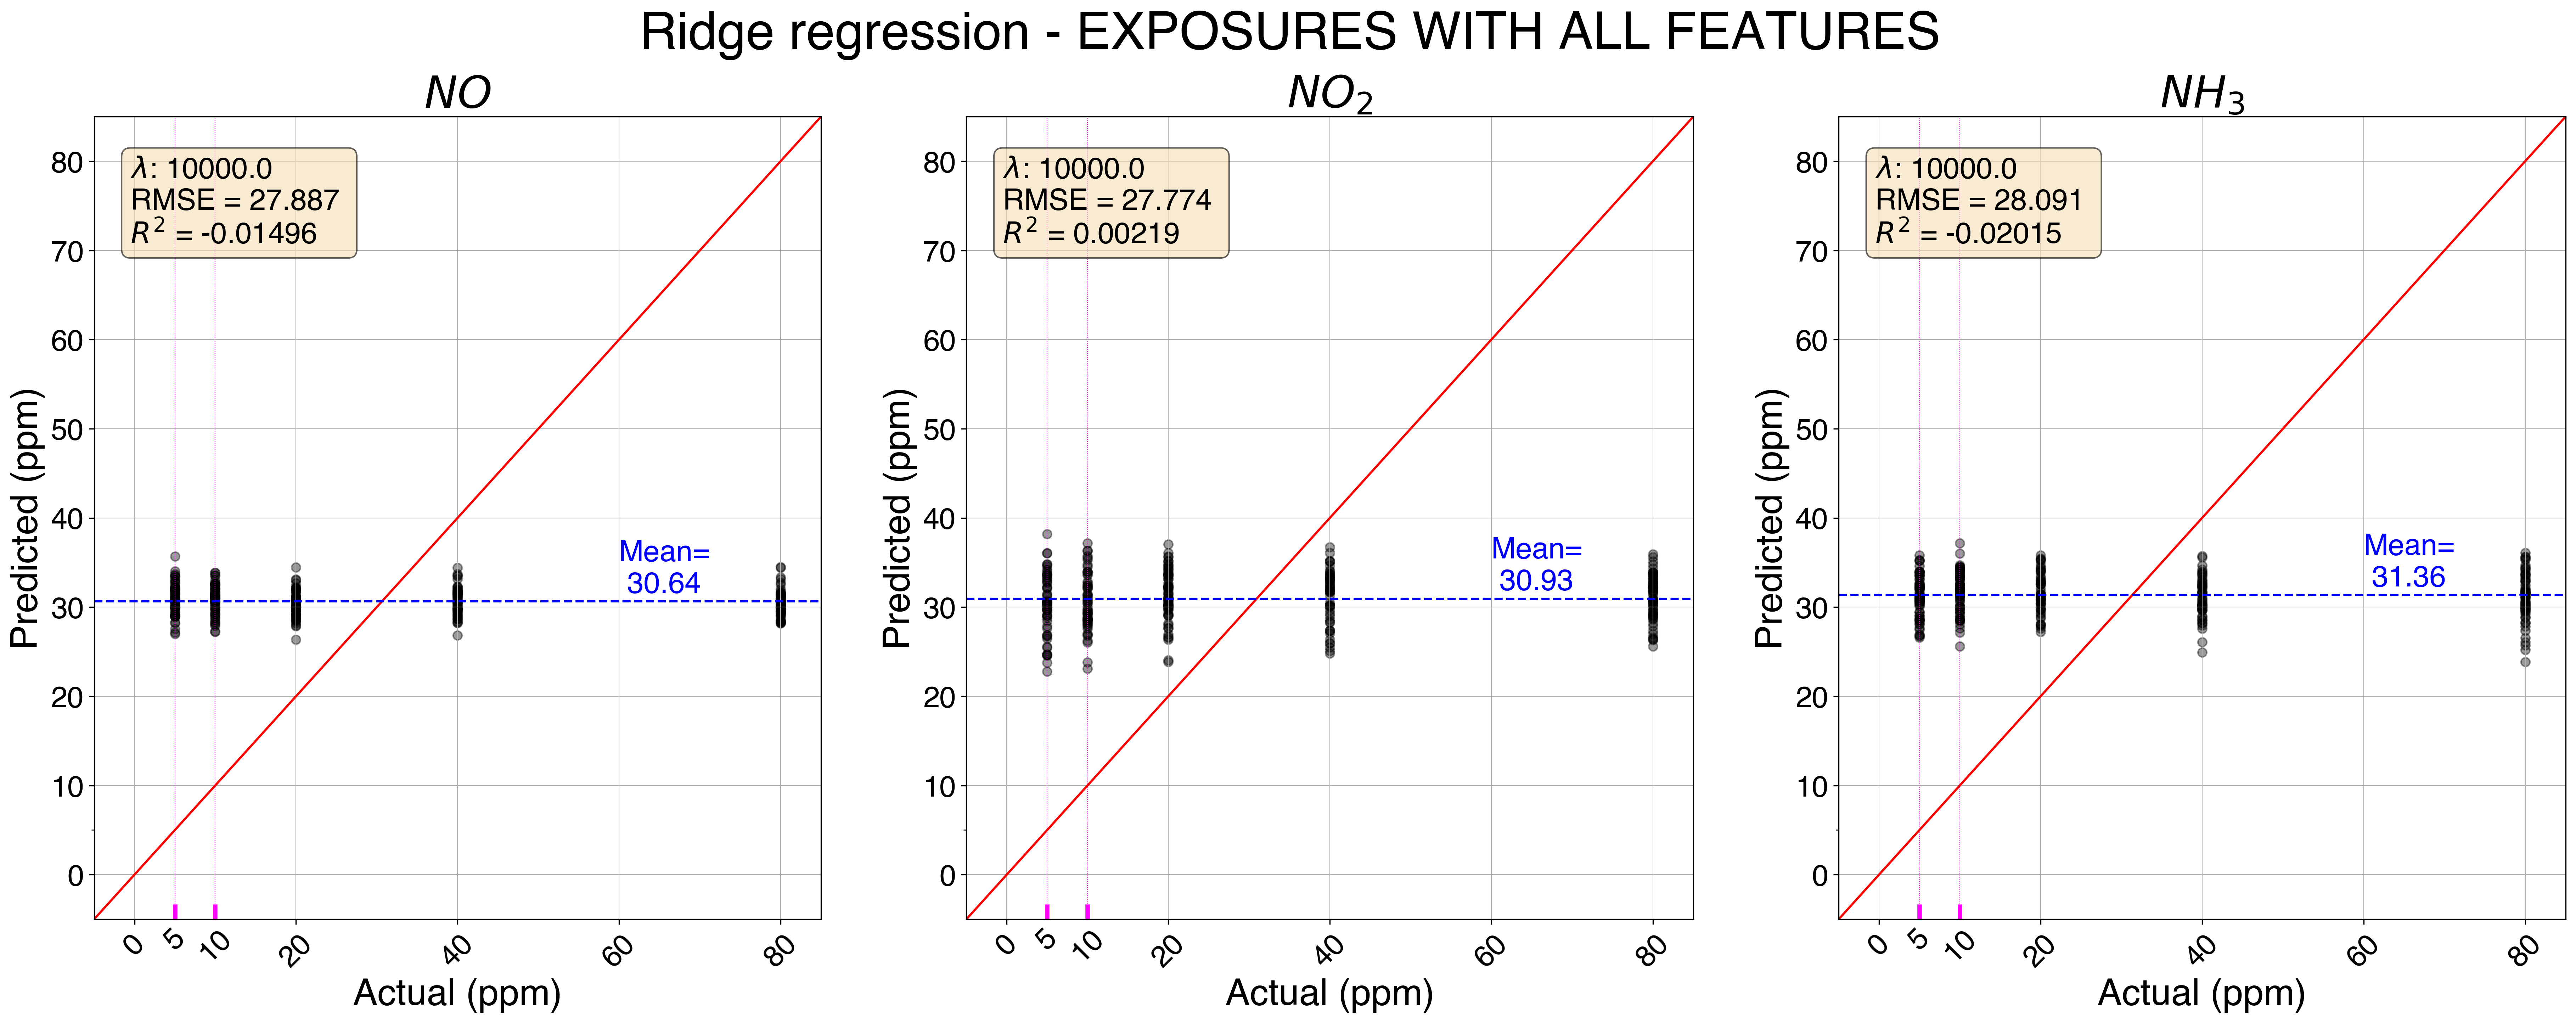
\includegraphics[width=1\linewidth]{../figures/ridge-act-vs-pred.png}
		\caption{}
		\label{fig:ridge-act-vs-pred} 
	\end{subfigure}
	
	\begin{subfigure}[t]{1\textwidth}
		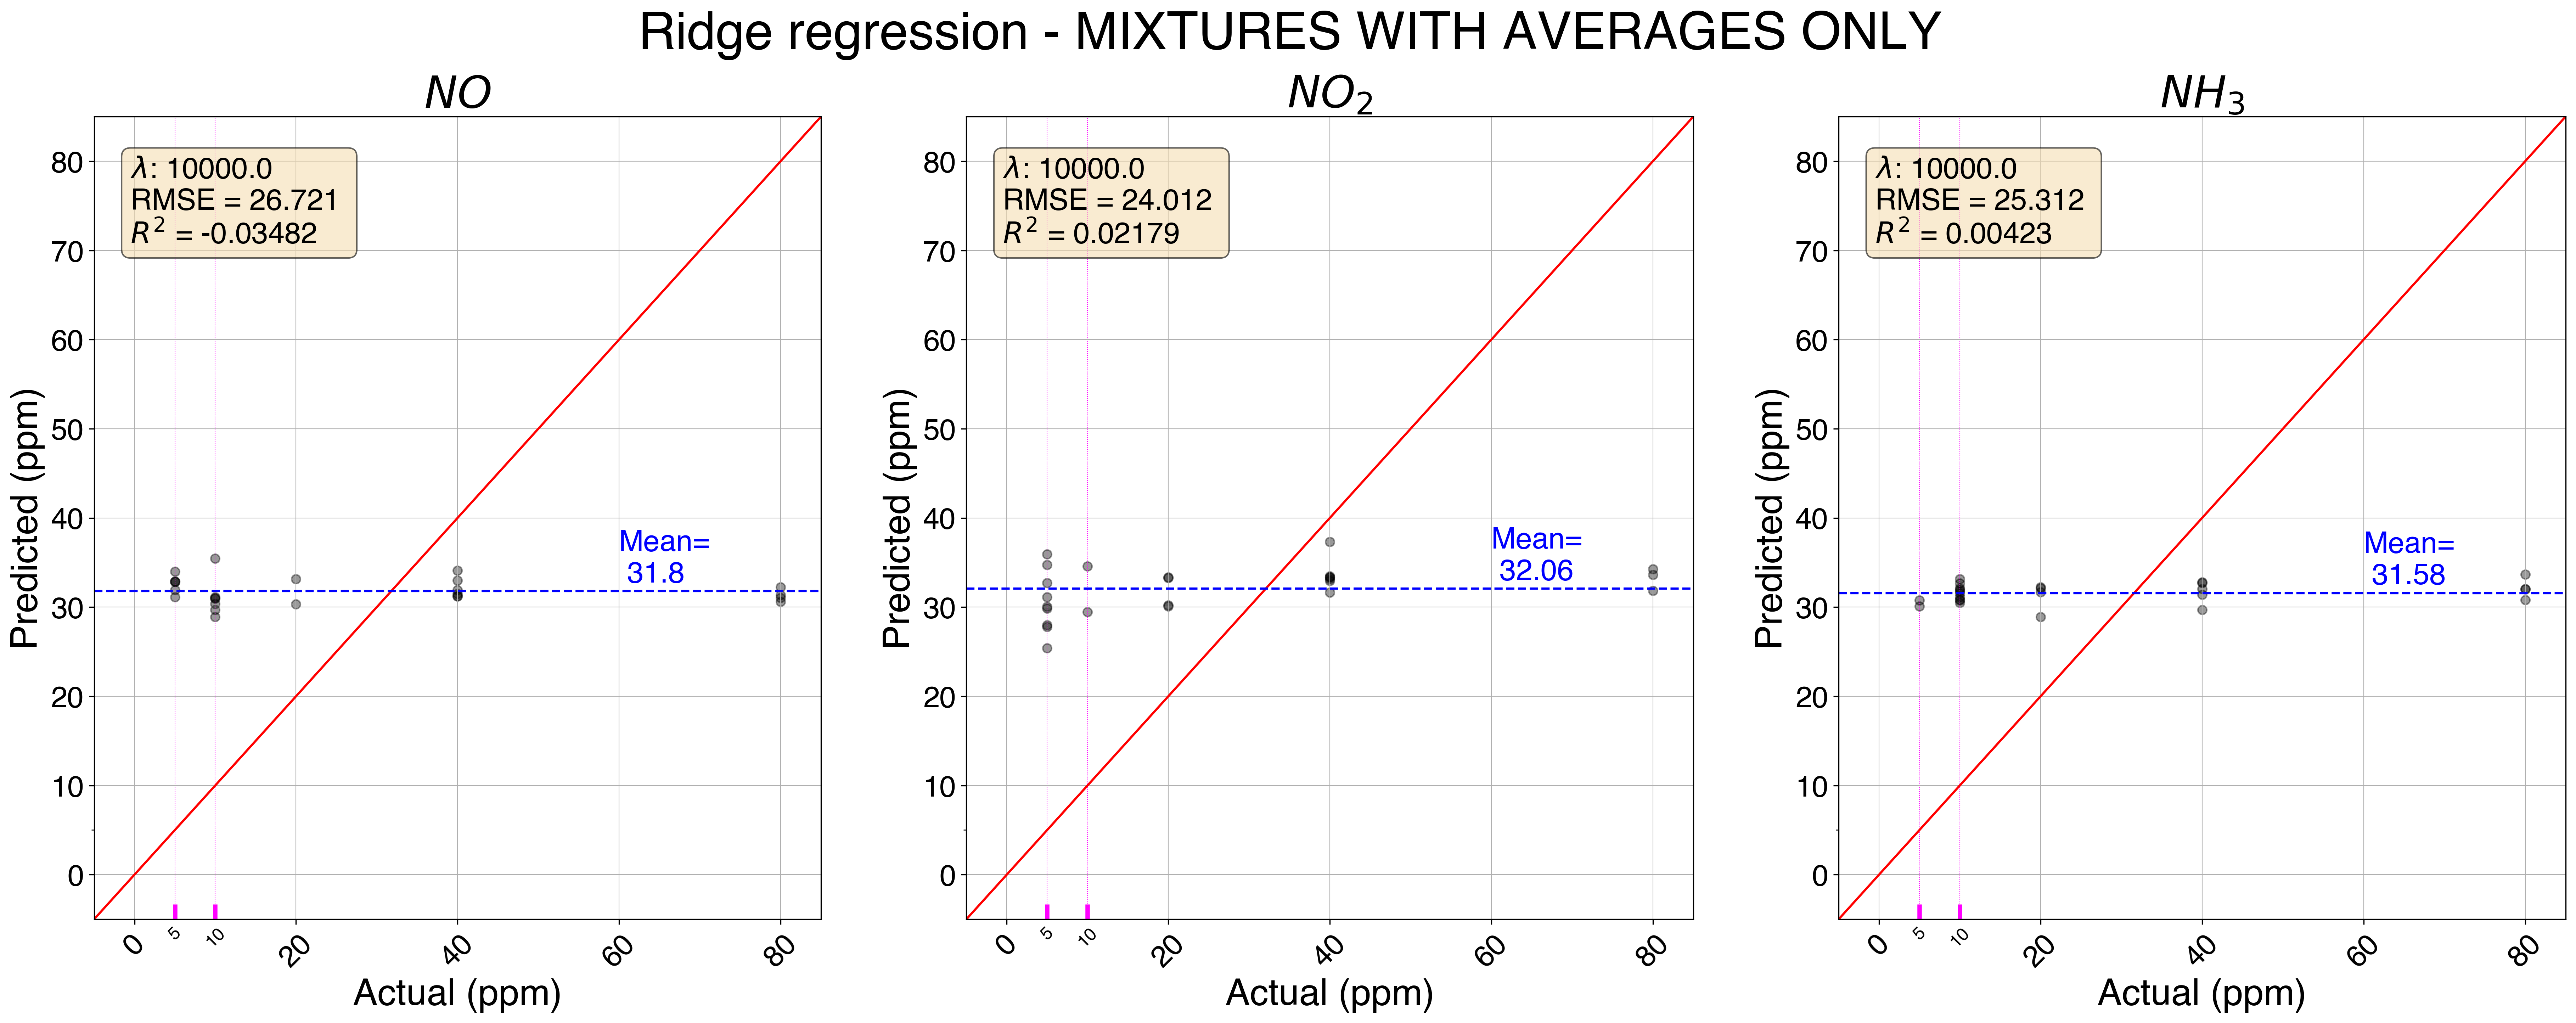
\includegraphics[width=1\linewidth]{../figures/ridge-act-vs-pred-avg-feat.png}
		\caption{}
		\label{fig:ridge-act-vs-pred-avg-feat}
	\end{subfigure}
	
	\caption{Ridge regression predictions for (a) slopes and averages through exposures and (b) only averaged average features through mixtures.}
	\label{fig:ridge-actual-vs-pred-both}
\end{figure}




